%% LyX 2.3.6 created this file.  For more info, see http://www.lyx.org/.
%% Do not edit unless you really know what you are doing.
\documentclass[10pt]{article}
\usepackage{helvet}
\renewcommand{\familydefault}{\sfdefault}
\usepackage[T1]{fontenc}
\usepackage[latin9]{inputenc}
\usepackage[a4paper]{geometry}
\geometry{verbose,tmargin=2cm,bmargin=4cm,lmargin=2cm,rmargin=2cm}
\usepackage{fancyhdr}
\pagestyle{fancy}
\setlength{\parskip}{6pt}
\setlength{\parindent}{0pt}
\usepackage{tcolorbox}
\usepackage{amsmath}
\usepackage{amsthm}
\usepackage{amssymb}
\usepackage{graphicx}

\makeatletter

%%%%%%%%%%%%%%%%%%%%%%%%%%%%%% LyX specific LaTeX commands.
%% A simple dot to overcome graphicx limitations
\newcommand{\lyxdot}{.}


%%%%%%%%%%%%%%%%%%%%%%%%%%%%%% User specified LaTeX commands.
\usepackage{tcolorbox}
\usepackage{amsthm}
\usepackage{lastpage}
\usepackage{fancyhdr}
\usepackage{accents}
\usepackage{titlesec}
\usepackage{marginnote}


\usepackage{enumitem}
\setlist{nolistsep}

\usepackage{tcolorbox}
\definecolor{light-blue}{cmyk}{0.24, 0.12, 0.0, 0.04, 1.00}

\title{CS7CS4 Week 8 Assignment}
\author{Neimhin Robinson Gunning 16321701}
\date{\today} 

%parskip shold take care of heading spacing
\titlespacing\section{0pt}{0pt}{0pt}
\titlespacing\subsection{0pt}{0pt}{0pt}
\titlespacing\subsubsection{0pt}{0pt}{0pt}



\setlength{\headheight}{40pt}

\makeatother

\begin{document}
\lhead{Neimhin Robinson Gunning (16321701)} \rhead{CS7CS4 Week 8 Assignment} 

\maketitle

\begin{tcolorbox}[colback=light-blue]
\begin{small} \textbf{DECLARATION:} I understand that this is an
\textbf{individual} assessment and that collaboration is not permitted.
I have read, understand and agree to abide by the plagiarism provisions
in the General Regulations of the University Calendar for the current
year, found at http://www.tcd.ie/calendar. I understand that by returning
this declaration with my work, I am agreeing with the above statement.
\end{small} 
\end{tcolorbox}

\bigskip{}


\section{(i)}

The results of a 2D convolution function applied to a single-channel
image, with two different kernels, are presented in Figure \ref{fig:A-200x200-RGB}.
The first kernel has the property that for a slice which is all one color multiplication with the kernel will be black (0).
This is not the case for the second kernel, so white regions of the image end up again being white/gray in the convolution output when convolved with $k_2$.
\begin{figure}
\begin{centering}

\includegraphics[width=0.25\textwidth]{fig/red_triangle200x200}~~~~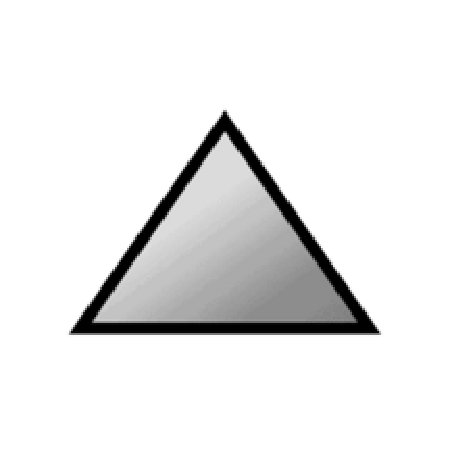
\includegraphics[width=0.25\textwidth]{fig/red_triangle-red-channel}
\par\end{centering}
\begin{centering}
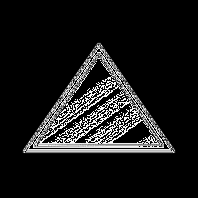
\includegraphics[width=0.25\textwidth]{fig/red_triangle-convolve-one}~~~~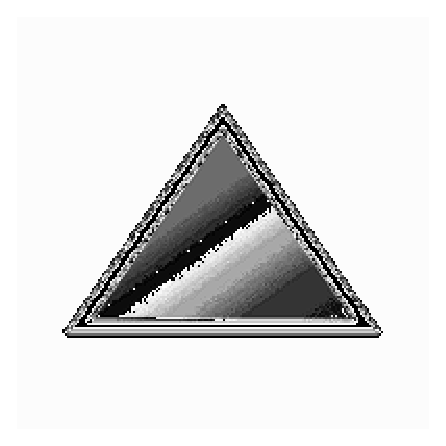
\includegraphics[width=0.25\textwidth]{fig/red_triangle-convolve-two}
\par\end{centering}
\begin{centering}
$k_{1}=\left[\begin{array}{ccc}
-1 & -1 & -1\\
-1 & 8 & -1\\
-1 & -1 & -1
\end{array}\right]$~~~~~~~~$k_{2}=\left[\begin{array}{ccc}
0 & -1 & 0\\
-1 & 8 & -1\\
0 & -1 & 0
\end{array}\right]$
\par\end{centering}
\caption{\label{fig:A-200x200-RGB}A 200x200 RGB image (top left) has green
and blue channels removed resulting in a grayscale image (top right).
The image is convolved with two kernels, $k_{1}$ (bottom left), and
$k_{2}$ (bottom right).}

\end{figure}


\section{(ii)}

\subsection{(ii) (a) model layers, kernels, channels}

In Figure \ref{fig:code} is the python source code for a CNN with 4 convolution layers.
The input to the model is a tensor with shape (32,32,3), i.e. an RGB
image with 32x32 pixels.

\begin{figure}
\includegraphics[width=1\textwidth]{fig/model_architecture\lyxdot py}
\caption{\label{fig:code}Source code of a ConvNet keras model.}
\end{figure}

The CNN layers of the model have the following structures:
\begin{enumerate}
\item (line 7): input=(32,32,3), number of kernels=16, kernel shape=(3,3,3),
output shape=(32,32,16)
\item (line 8): input=(32,32,16), number of kernels=16, kernel shape=(3,3,16),
output shape=(16,16,16)
\item (line 9): input shape=(16,16,16), number of kernels=32, kernel shape=(3,3,16),
output shape=(16,16,32)
\item (line 10): input shape=(16,16,32), number of kernels=32, kernel shape=(3,3,32),
output shape=(8,8,32)
\end{enumerate}
The next layer is a dropout layer which randomly sets on average 50\%
of its inputs to 0 and leaves the rest of the inputs the same. Its
input and output shape is (8,8,32). The next layer simply unravels
the (8,8,32) tensor into an array of length $2048=8\cdot8\cdot32$.
The final layer `Dense' layer first computes 10 separate linear combinations of length 2048 input vector.
The output of this `Dense' layer is just the `softmax'
function applied to the vector of ten linear combinations,
$[ z_1, \ldots, z_{10}]$.
A definition of the softmax function is given in Equation \ref{eq:softmax}
and a description of the final output of the model is given in Equation \ref{eq:out-proba}.

\begin{equation}
    \label{eq:softmax}
    \text{softmax}(z_i) = \frac{e^{z_i}}{\sum_{j=1}^{10} e^{z_j}}
\end{equation}

\begin{equation}
    \label{eq:out-proba}
    \text{output of dense layer} = [ \text{softmax}(z_1), \text{softmax}(z_2), \ldots, \text{softmax}(z_{10}) ] 
\end{equation}


\subsection{(ii) (b) (i)}
Keras reports that model given by the code in Figure \ref{fig:code} has 37146 total parameters, all of which are trainable.
The final Dense layer has the most parameters, namely $2048\cdot10+10=20490$.
The number of parameters in a convolution layer is determined by the kernel size and the number of filters and the number of channels,
$$\text{no. params}=(k_w\cdot k_h\cdot c + 1)\cdot f$$,
where $k_w$ and $k_h$ are the kernel dimensions, $c$ is the number of filters, there's 1 bias for each kernel, and $f$ is the number of kernels/filter.
However, the number of parameters in a Dense layer is determined by the input and output sizes.
Since the input dimension for the Dense layer is quite large (2048), this layer ends up having more
parameters than any of the convolution layers.

The model's accuracy is markedly better on the training data than on the test data.
On the training data the model has an accuracy of 57\%, but on the test data it is 48\%.
A simple baseline which always predicts the most frequent class achieves an accuracy of 10\%,
which is natural considering the test set is balanced and there are ten classes,
and the average $F_1$-score of the baseline classifier across the classes in 0.018.
The ConvNet is much better than the `most\_frequent' baseline.

\subsection{(ii) (b) (ii)}
The history of loss and accuracy of the model trained on 5K samples over 20 epochs is presented in Figure \ref{fig:iibii-acc-loss}.
Generally improvements to loss and accuracy after each epoch are diminishing.
The progression of loss and accuracy when training on 5K samples shows that the train loss and train accuracy
more or less improve monotonically, but the test loss and accuracy start to plateau earlier at around 10 epochs.
The process of the train and val scores diverging on subsequent epochs is an indicator of overfitting.

\begin{figure}
    \begin{centering}
        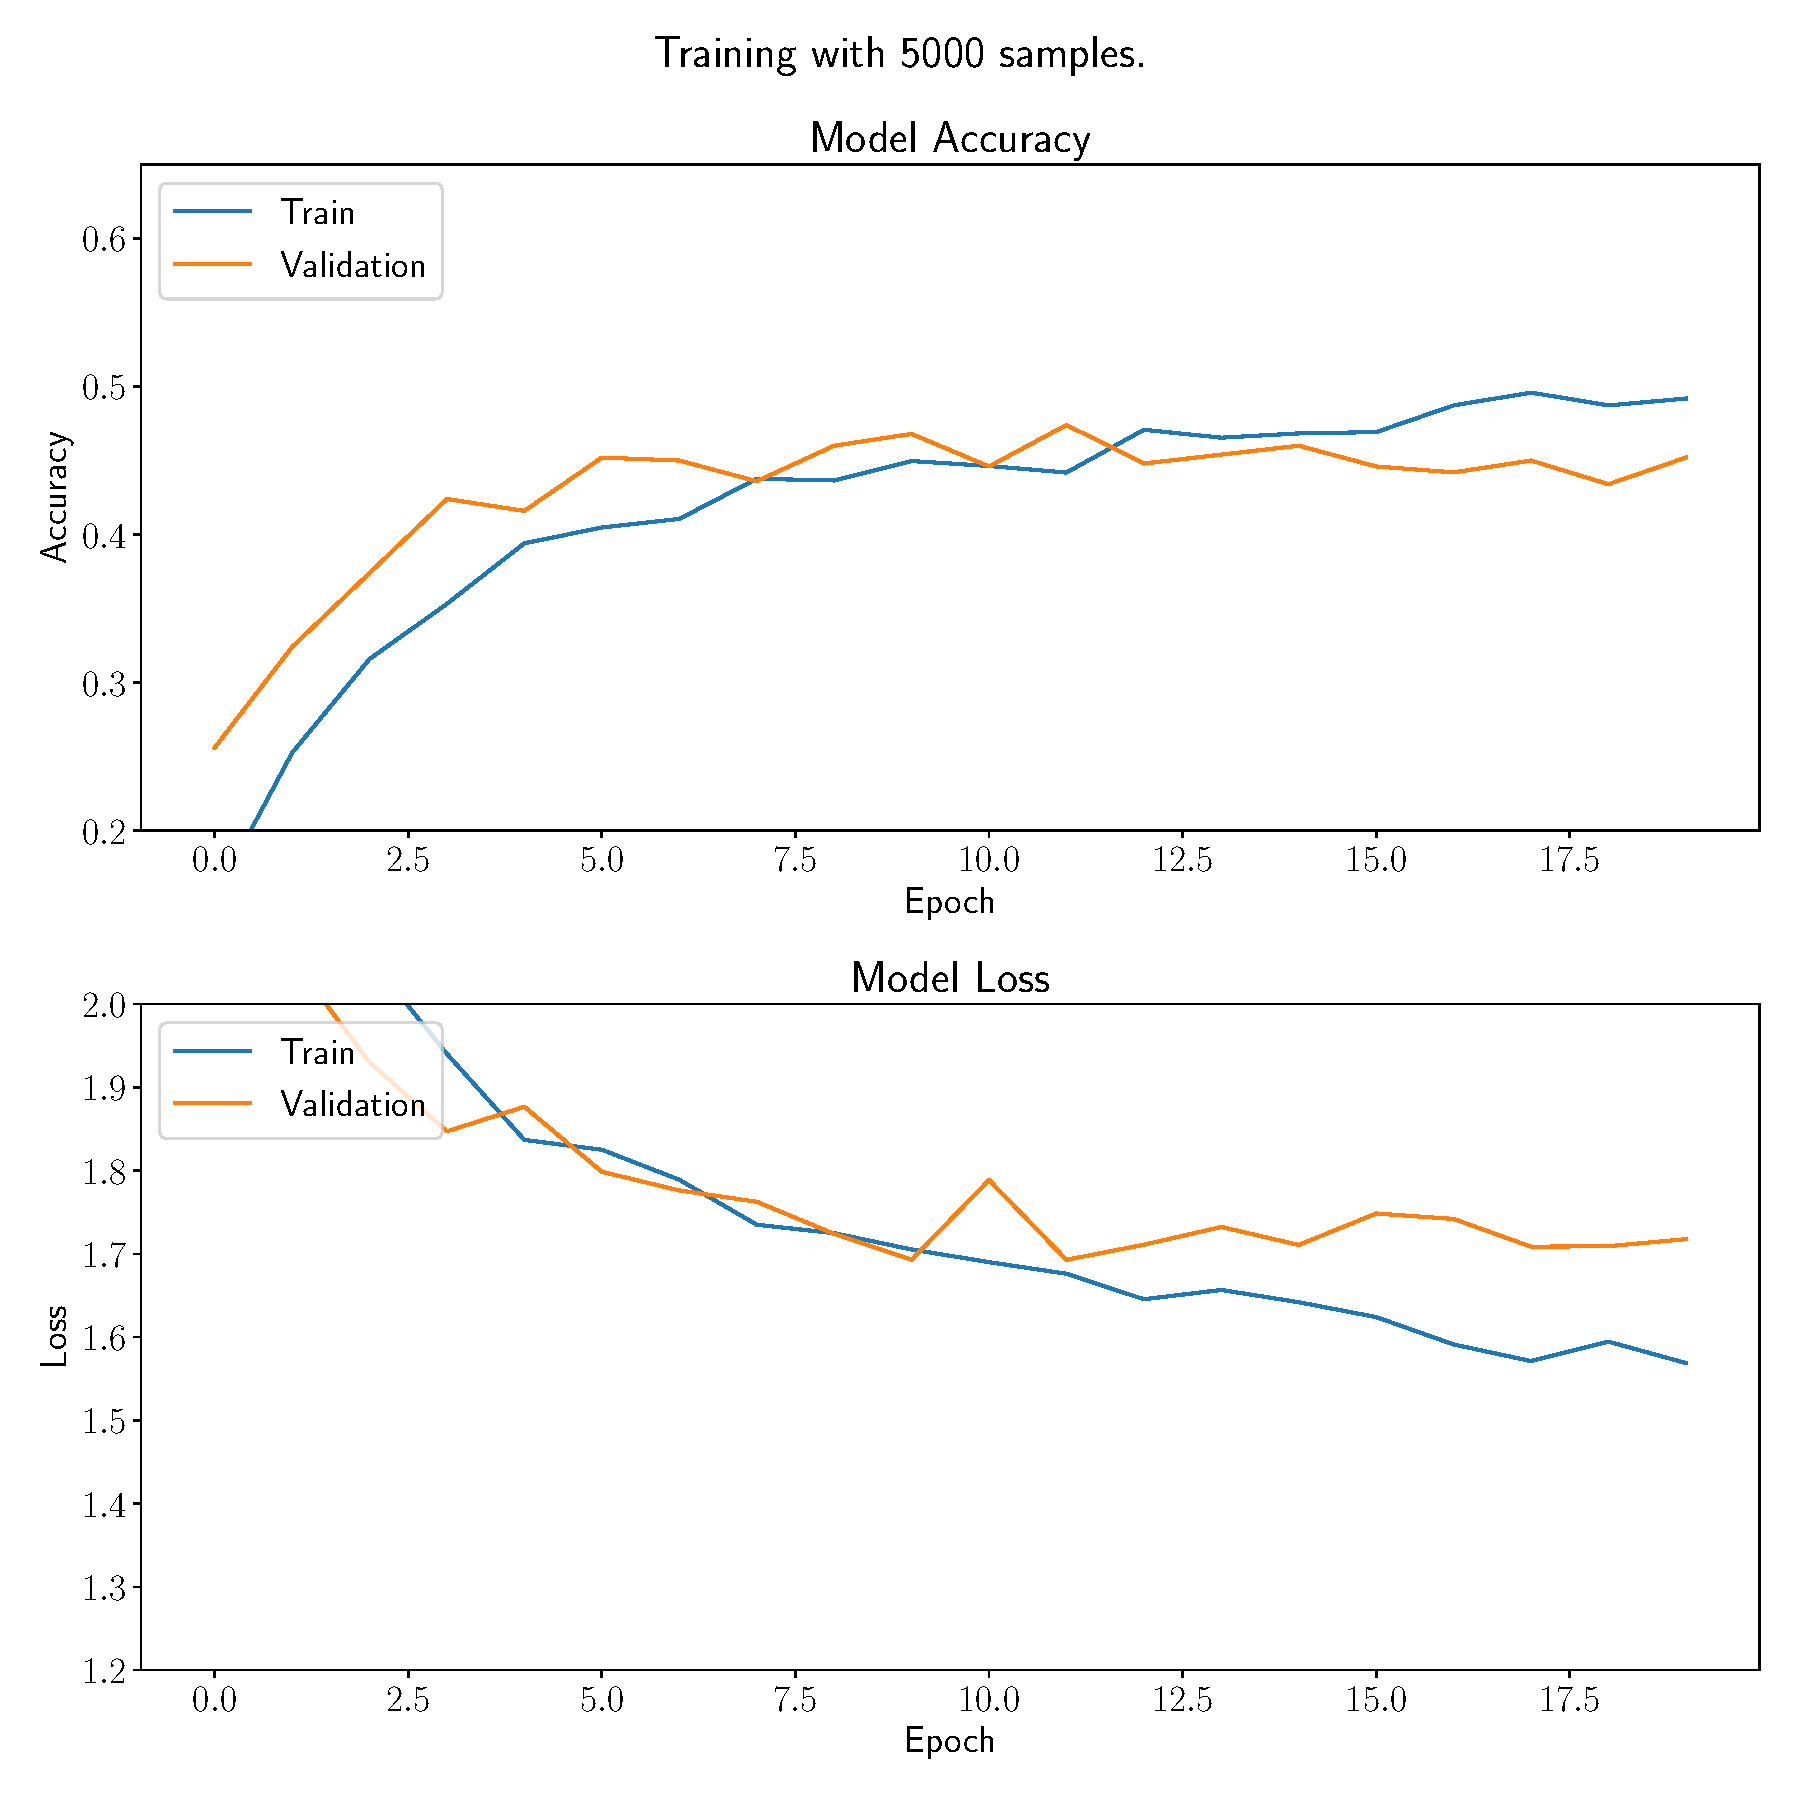
\includegraphics[width=0.49\textwidth]{exp/iibiii/5000.acc-loss.pdf}
    \par\end{centering}
    \caption{\label{fig:iibii-acc-loss}
    A comparison of accuracy/loss on training/test data from
    epochs 1 to 20 when trained on 5K training samples with $L_1=0.001$.}
\end{figure}

\subsection{(ii) (b) (iii)}
Figure \ref{fig:iibiii-acc-loss} presents plots of the `histories' of the training losses and accuracies on training/validation data
for a sequence of models trained on 5K, 10K, 20K, and 40K training samples.
Naturally, the model with most training data achieves the lowest loss and highest accuracy on the validation data.
For 5K training samples the gap between training and validation scores starts to increase after about 10 epochs, indicating over-fitting.
In particular, by the 20th epoch the accuracy on the training data is higher than the accuracy on the validation data
and the loss on the training data is lower than the loss on the validation data.
With 40K training samples the scores do not indicate significant over-fitting.
Generally the divergence of train and val scores is less with more training data.

The general reading we can take from Figure \ref{fig:iibiii-acc-loss}
is that more training data allows us to train for more epochs without over-fitting,
or without over-fitting as much.

\begin{figure}
    \begin{centering}
        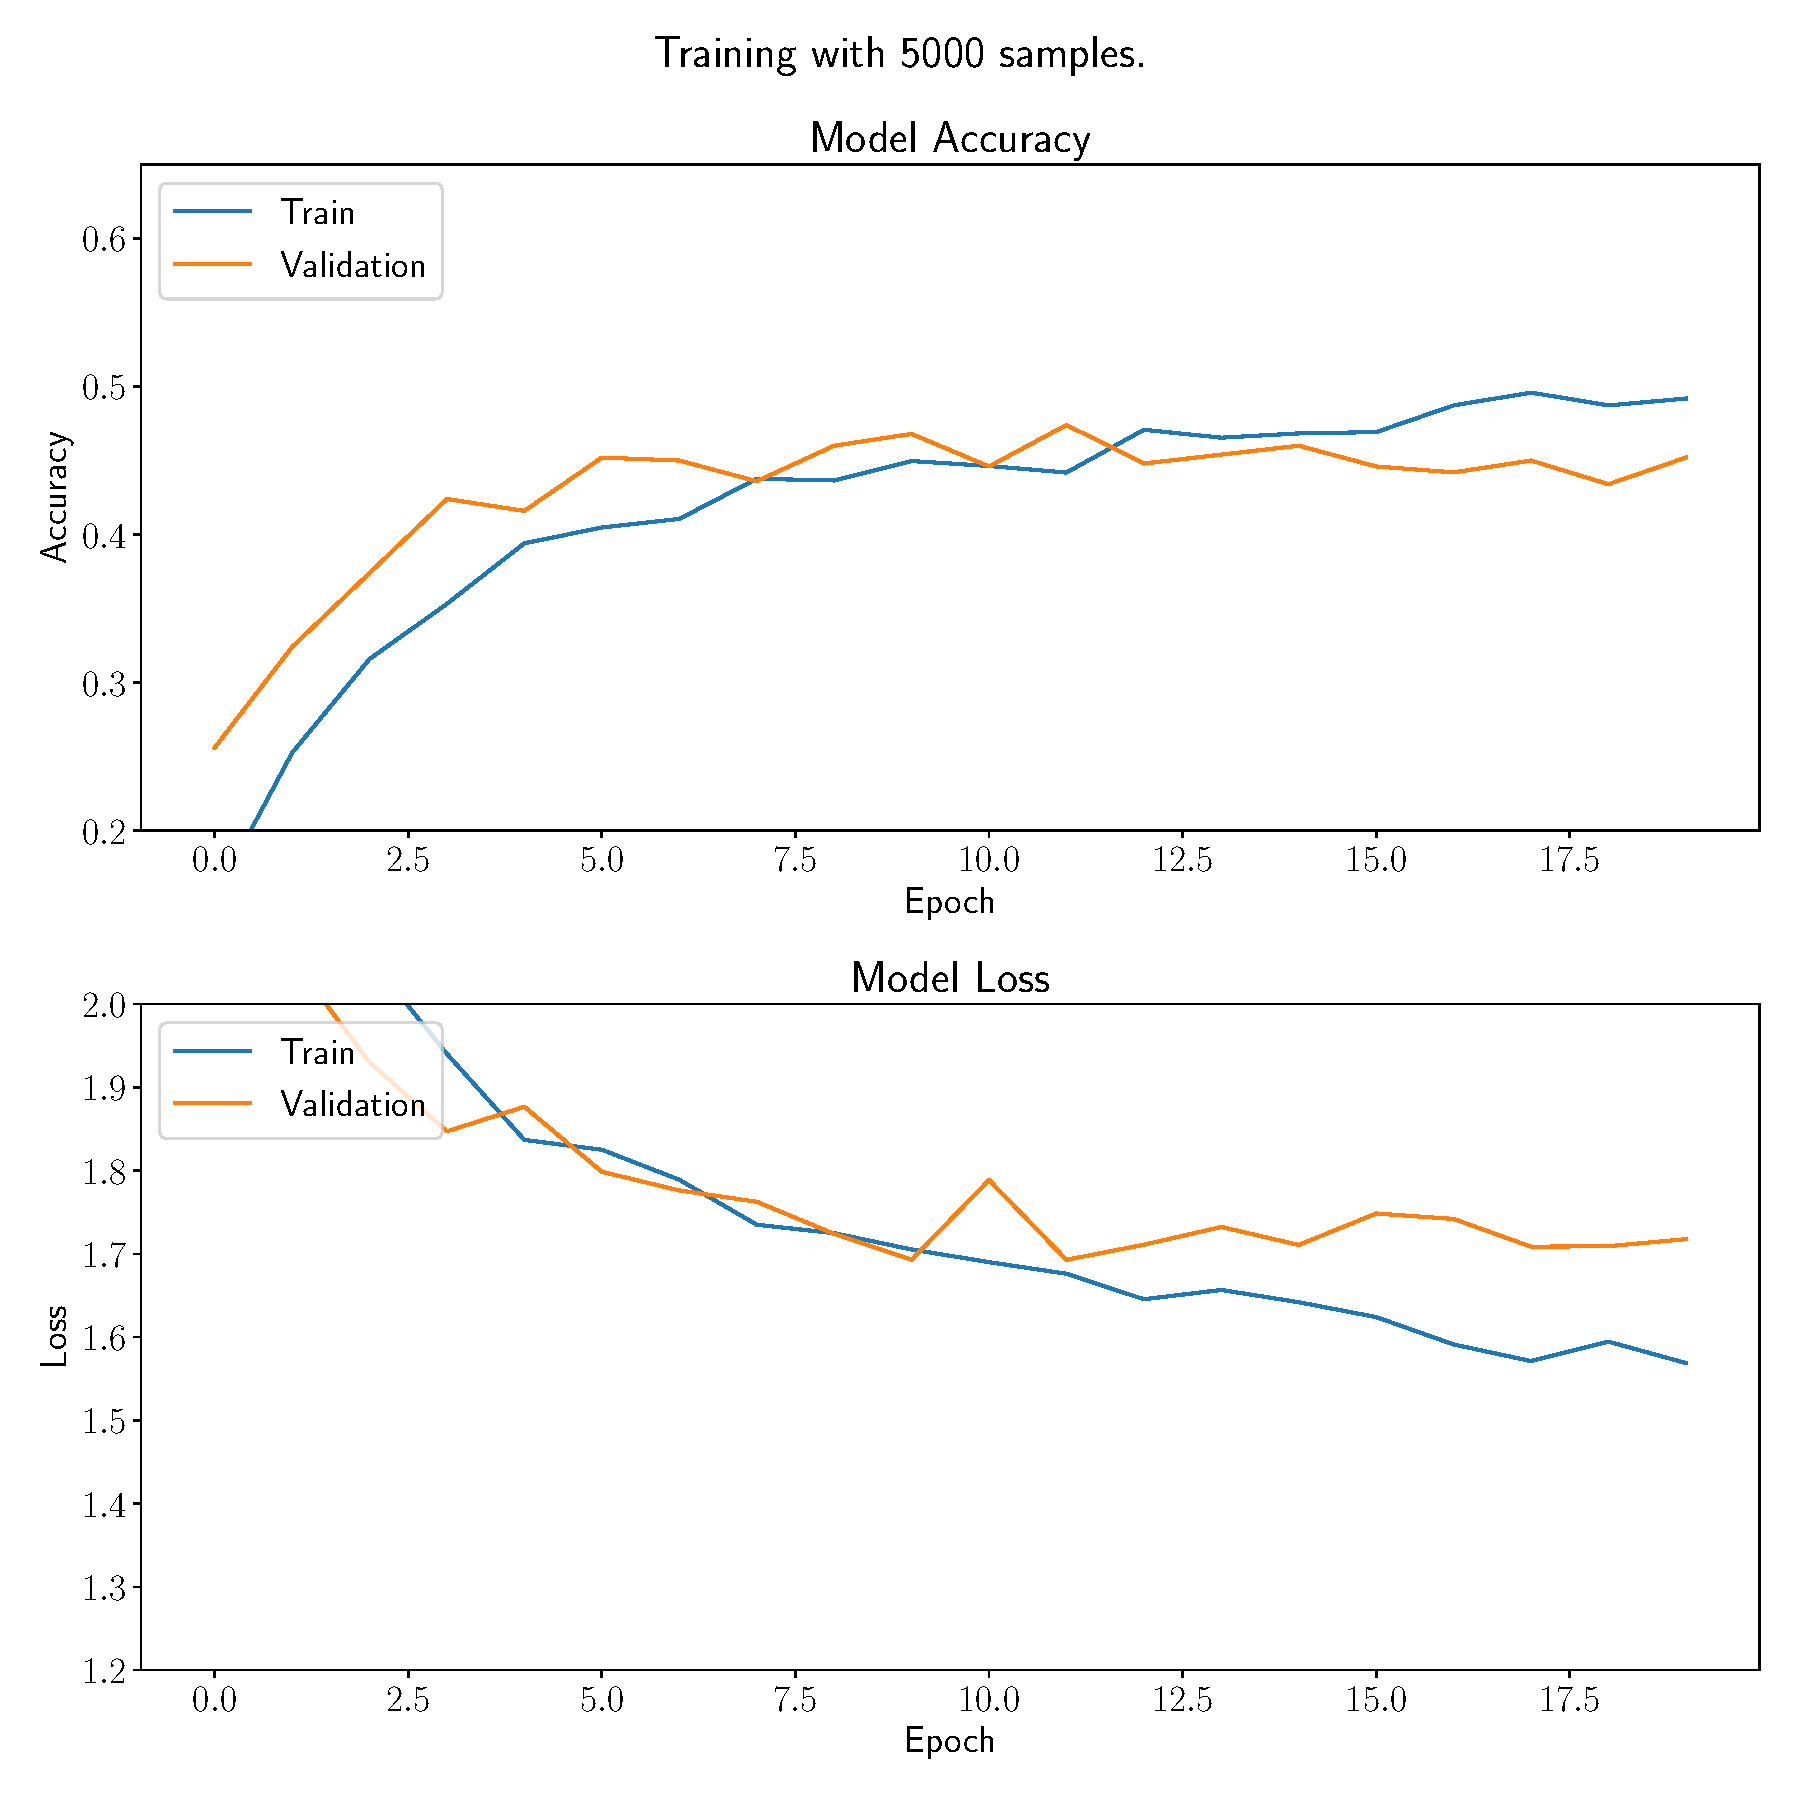
\includegraphics[width=0.49\textwidth]{exp/iibiii/5000.acc-loss.pdf}
        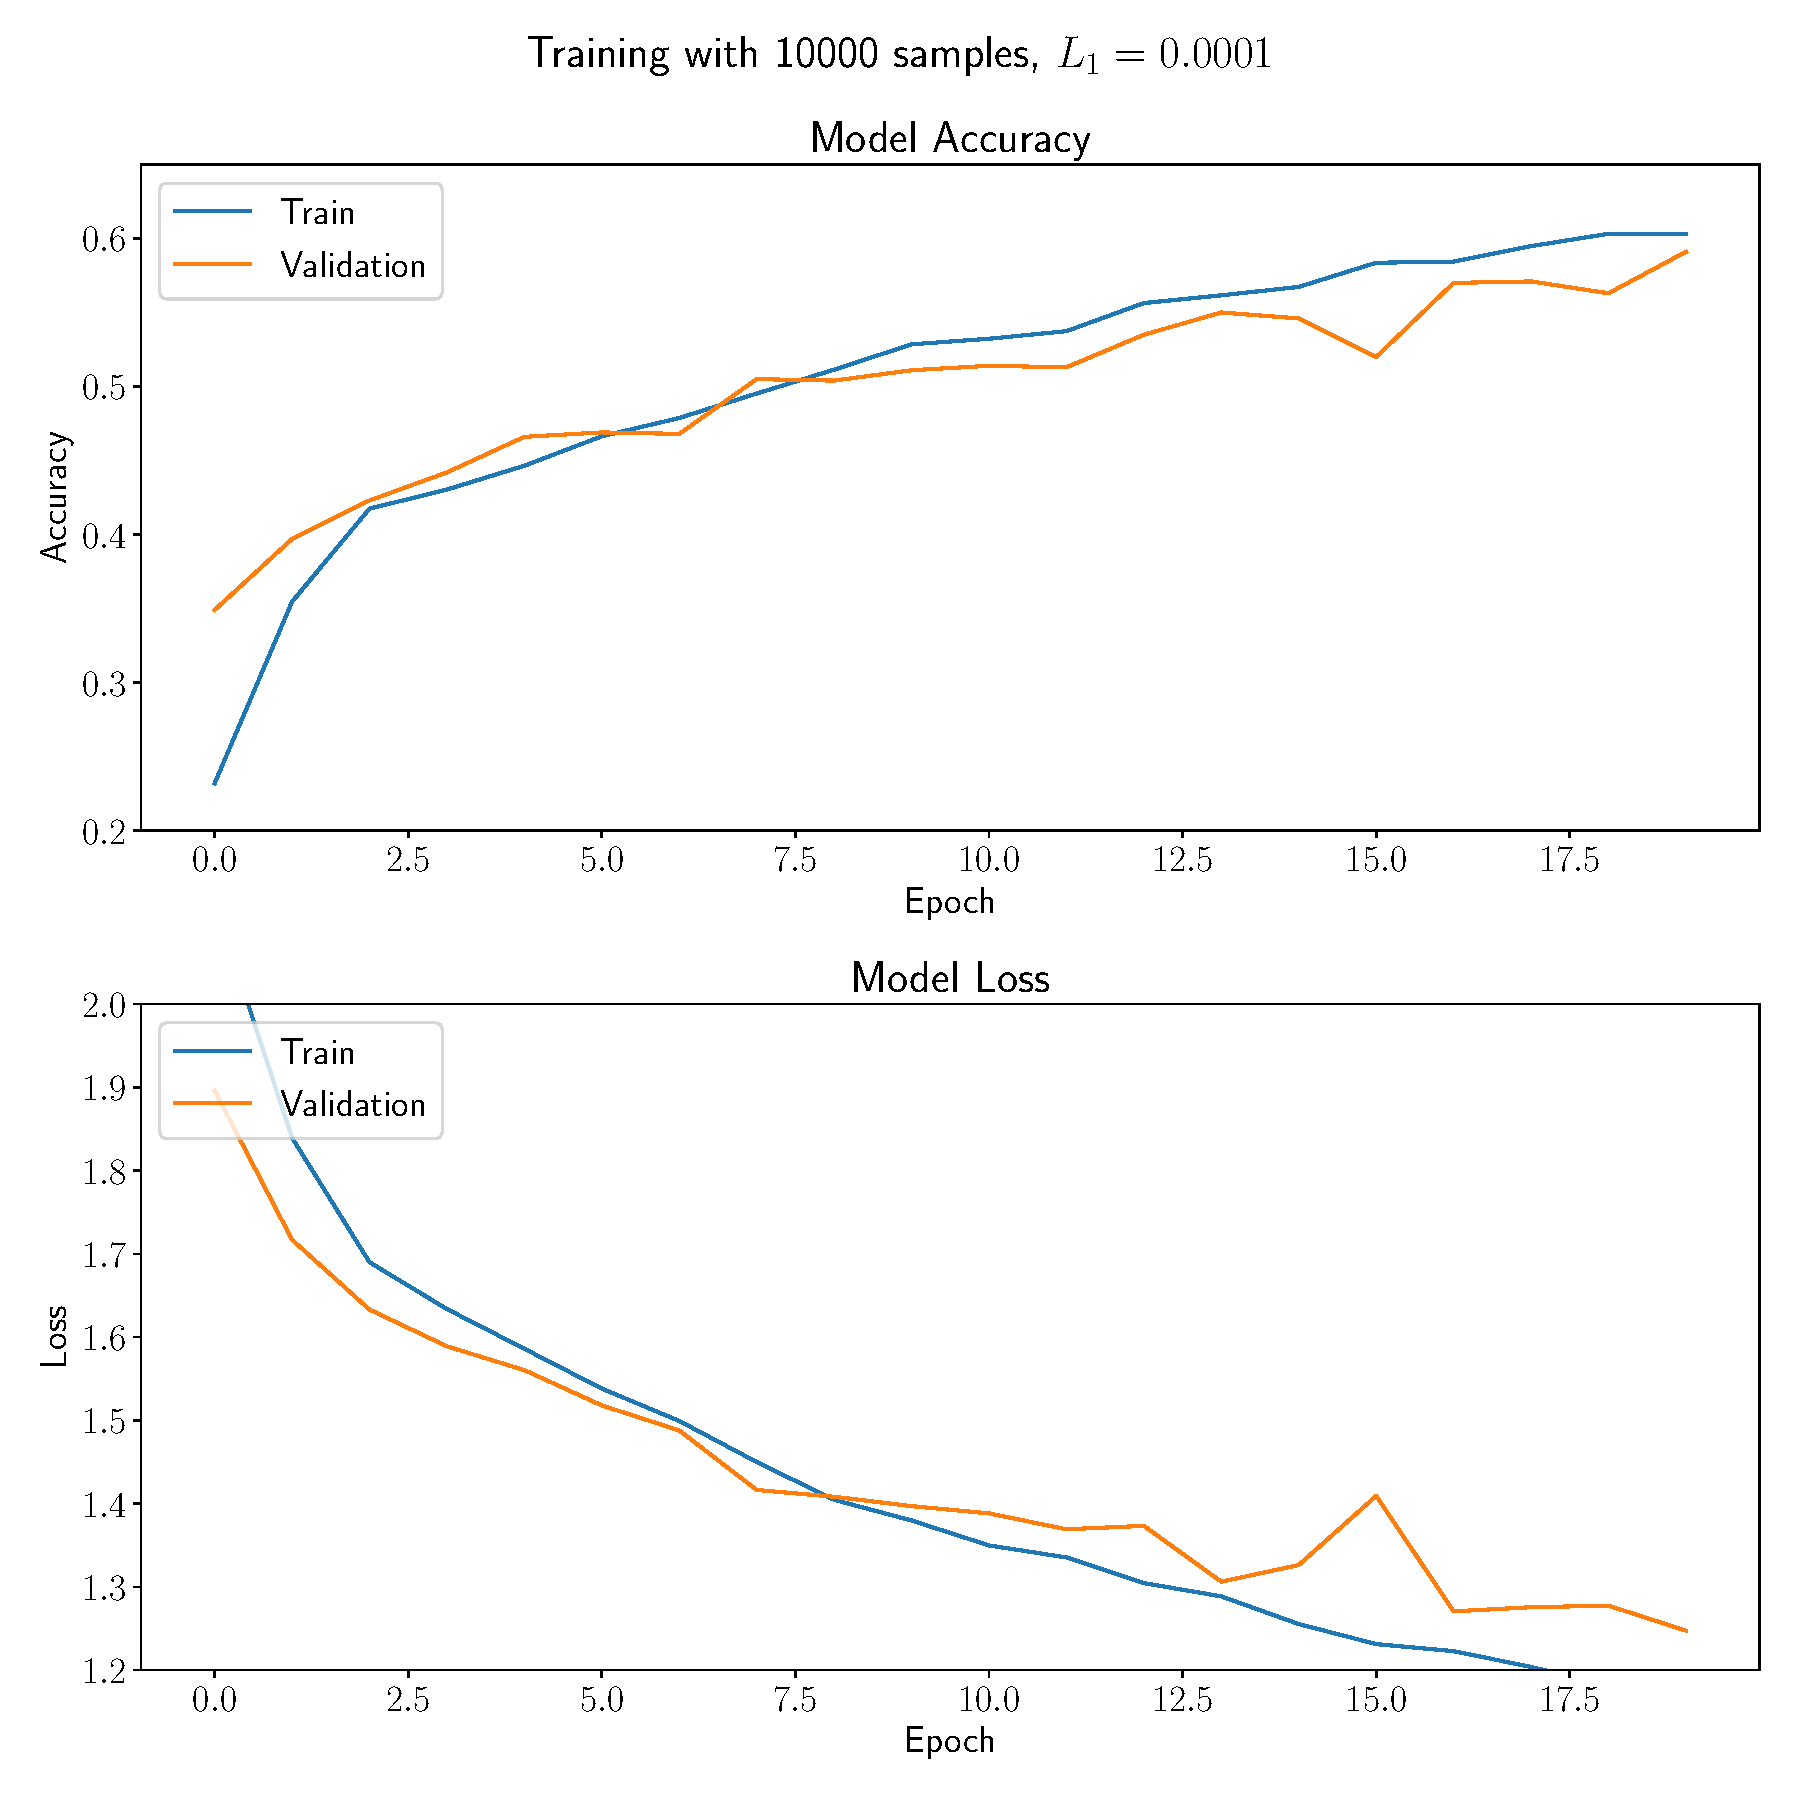
\includegraphics[width=0.49\textwidth]{exp/iibiii/10000.acc-loss.pdf}
    \par\end{centering}
    \begin{centering}
        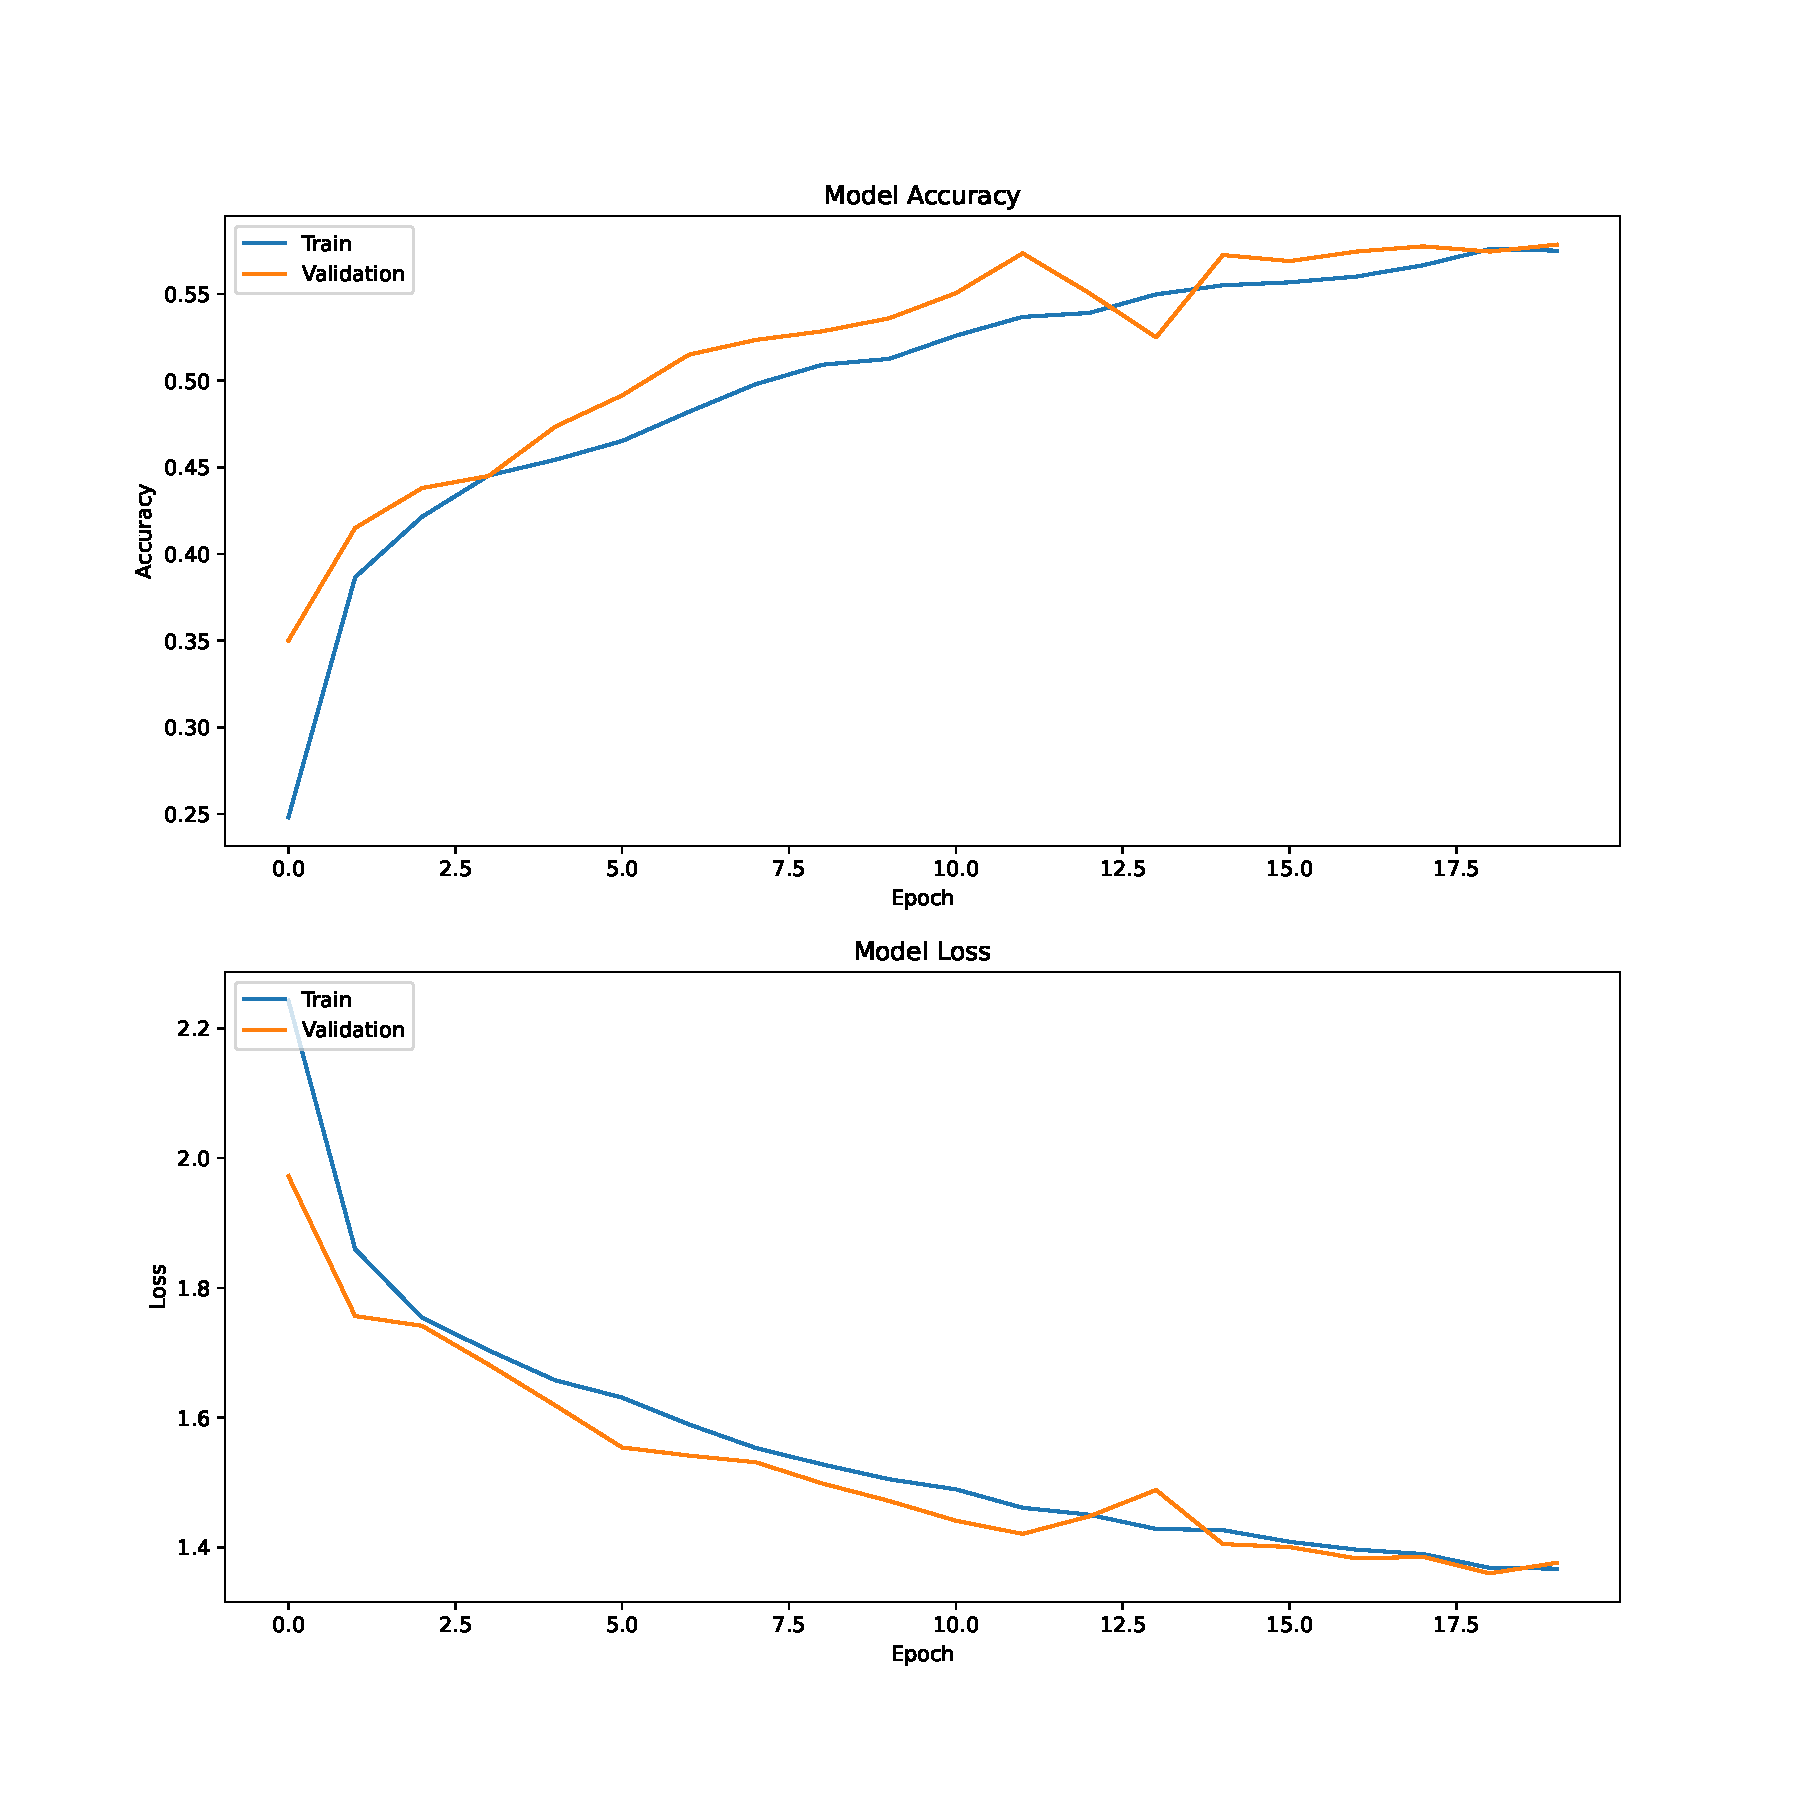
\includegraphics[width=0.49\textwidth]{exp/iibiii/20000.acc-loss.pdf}
        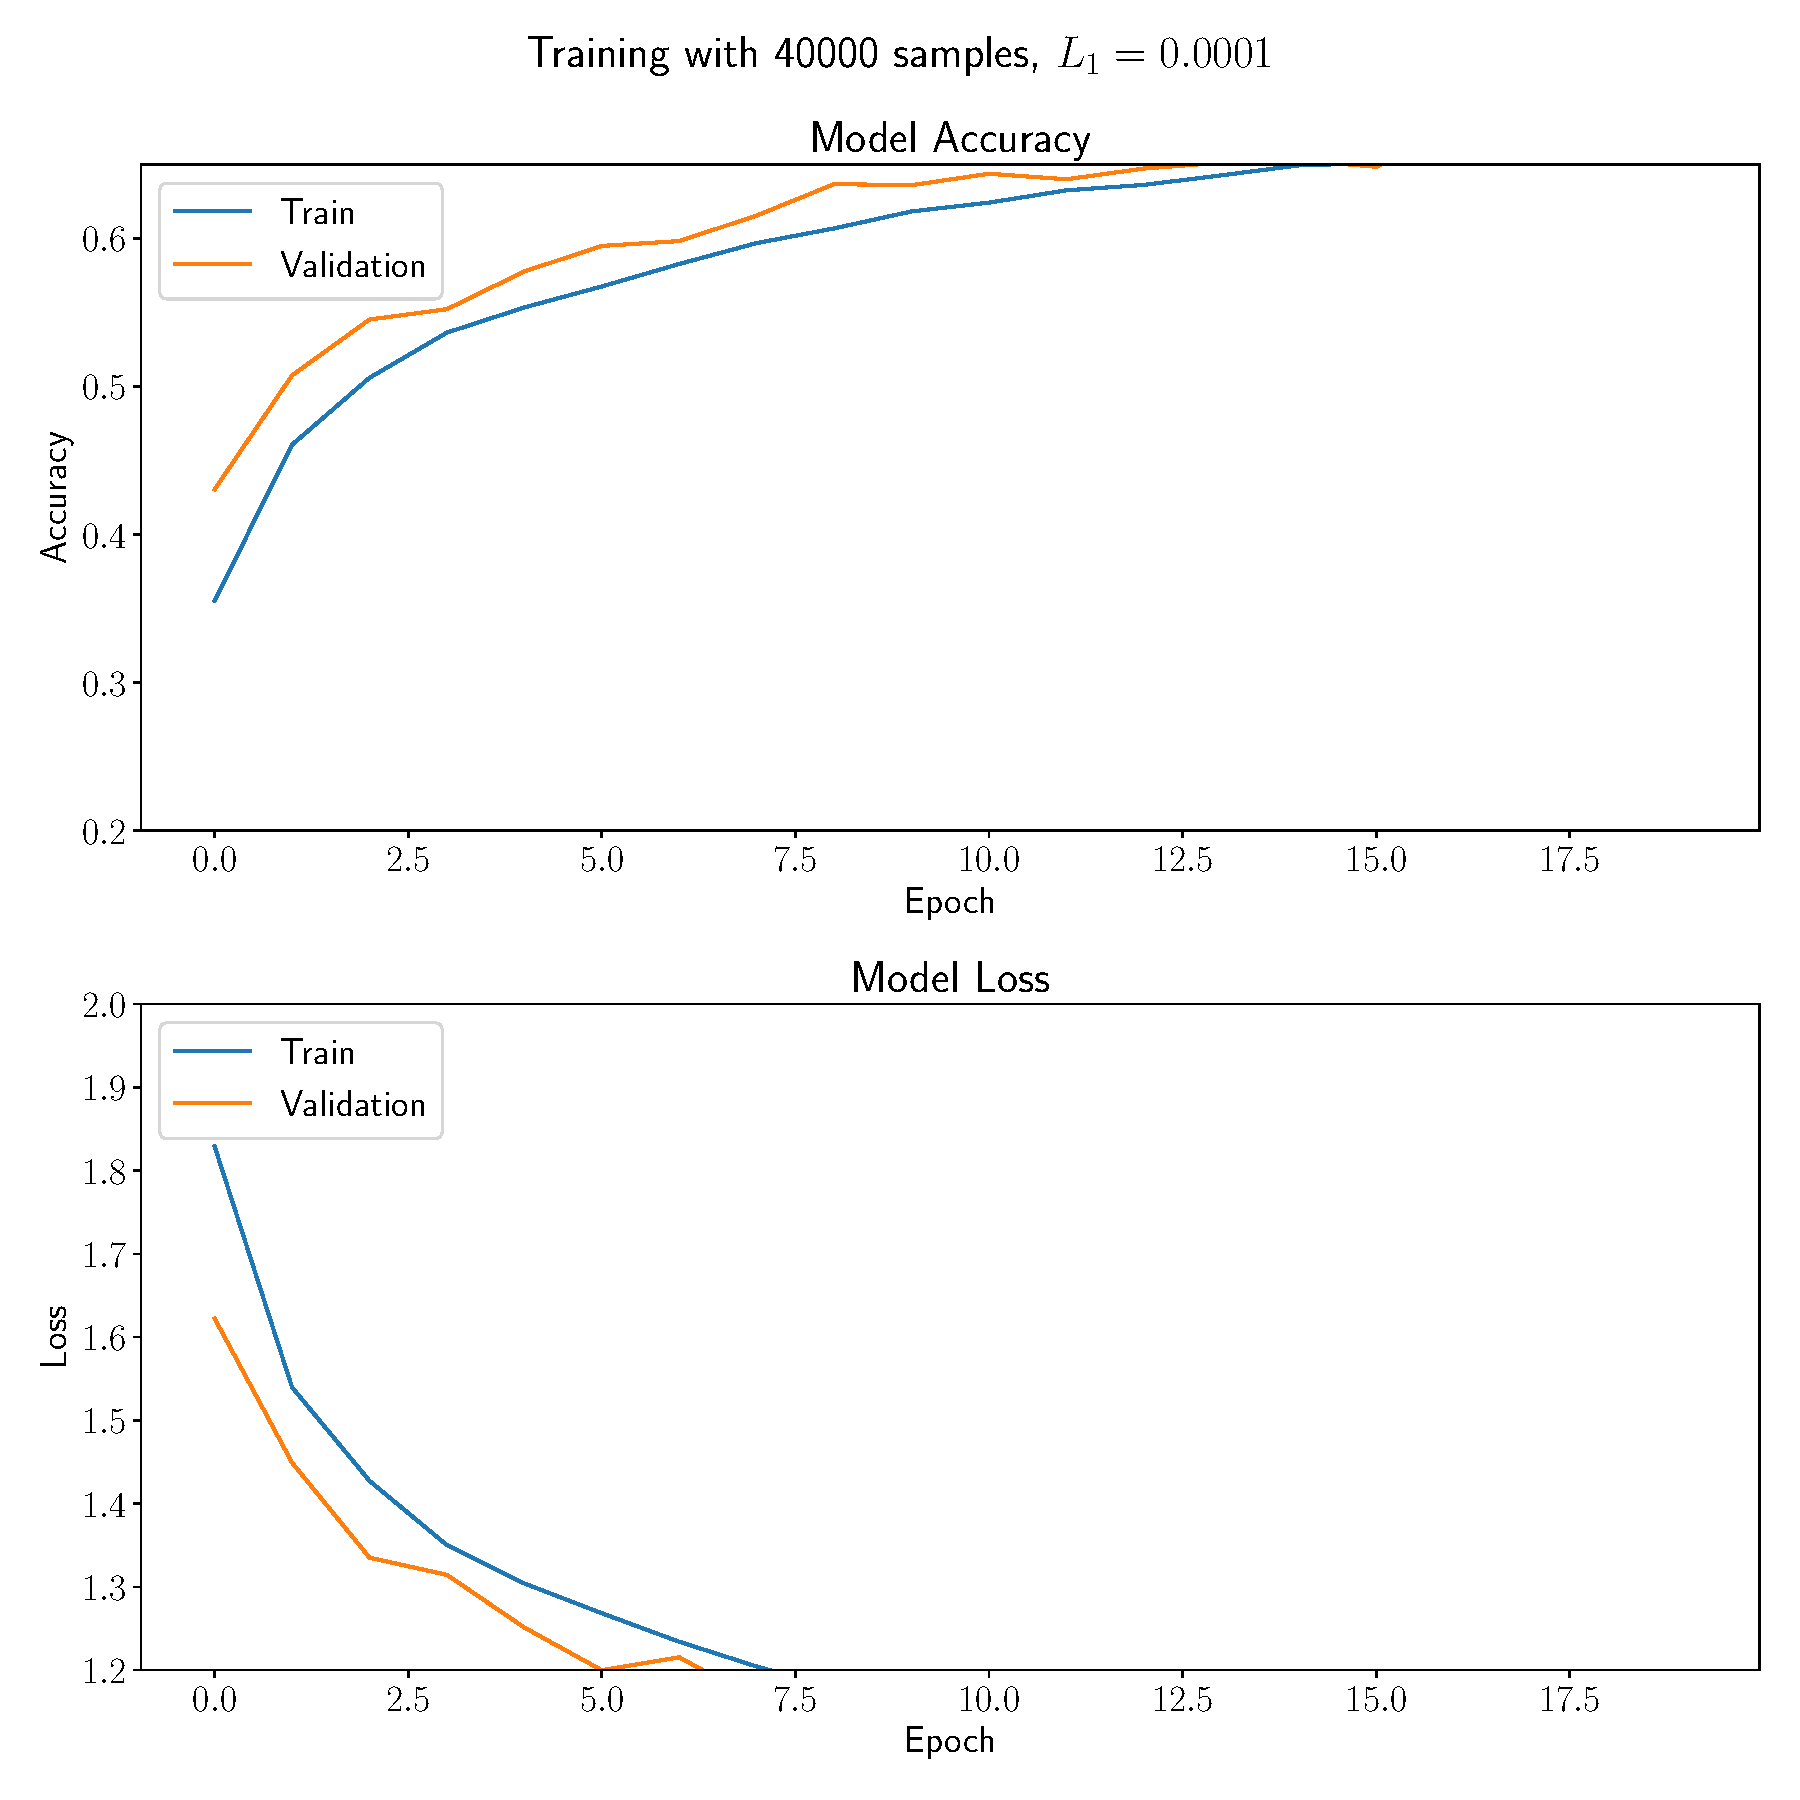
\includegraphics[width=0.49\textwidth]{exp/iibiii/40000.acc-loss.pdf}
    \par\end{centering}
    \caption{\label{fig:iibiii-acc-loss}
    A comparison of accuracy/loss on training/test data from
    epochs 1 to 20 for different quantities
    of training data, 5K, 10K, 20K and 40K.  Each model is trained with $L_1=0.001$.}
\end{figure}

\begin{figure}
    \begin{centering}
        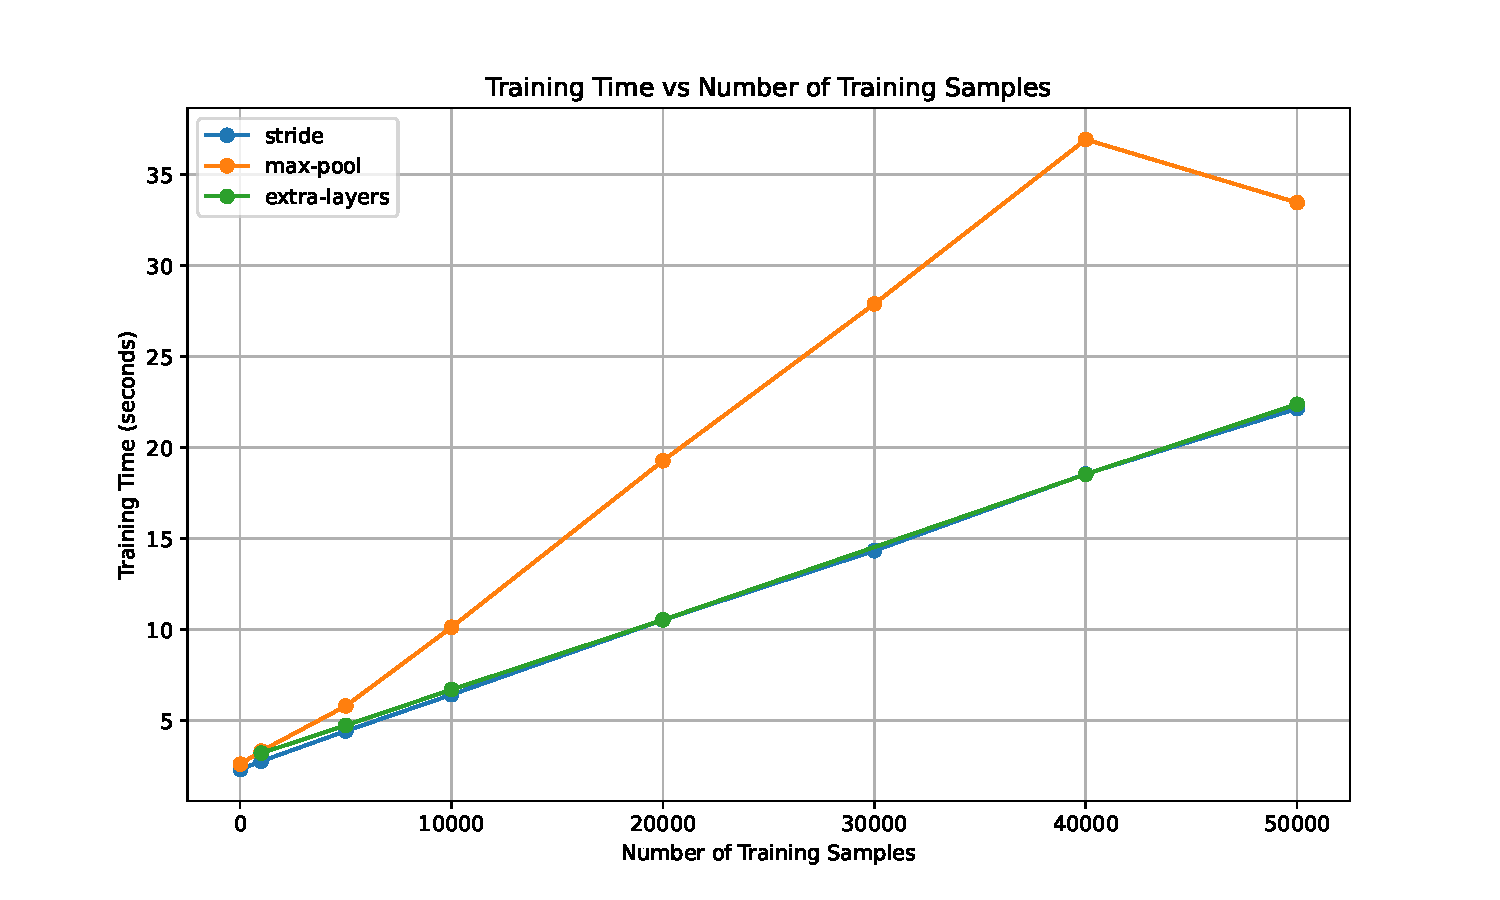
\includegraphics[width=0.7\textwidth]{fig/timing-comparison.pdf}
    \par\end{centering}
    \caption{\label{fig:timing}The amount of time needed to train the ConvNet for 20 epochs is 
    plotted against thet number of training samples used. The relationship is linear. The strided architectures with different depths have similar training times,
    but the max-pooling architecture is significantly slower to train.}
\end{figure}

In Figure \ref{fig:size-v-acc} we compare the accuracy on train and test sets
for a sequence of models with different training set sizes.
The general trend is that the difference between train and test accuracy decreases
as the amount of data used is increased, and at the same time increasing the amount of data
increases the ultimate test accuracy.

\begin{figure}
    \begin{centering}
        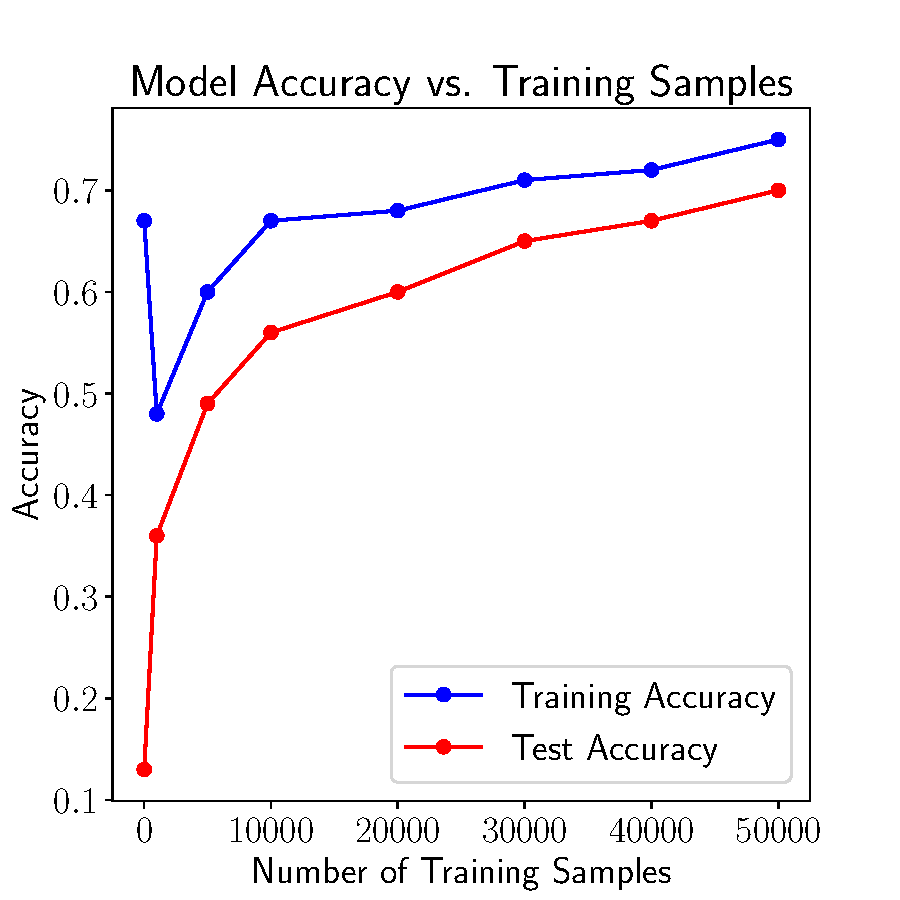
\includegraphics[width=0.49\textwidth]{fig/size-v-accuracy.pdf}
    \par\end{centering}
    \caption{\label{fig:size-v-acc}
    A comparison of accuracy on the train and test sets for different sizes of training data, 10, 1K, 5K, 10K, 20K, 40K, and 50K.}
\end{figure}

\subsection{(ii) (b) (iv)}
In Figure \ref{fig:l1-v-acc} we can see the effect of changing $L_1$ on the train and test accuracies of the model.
The optimal choice for $L_1$ when training on 20K samples seems to be around 0.00001.

\begin{figure}
    \begin{centering}
        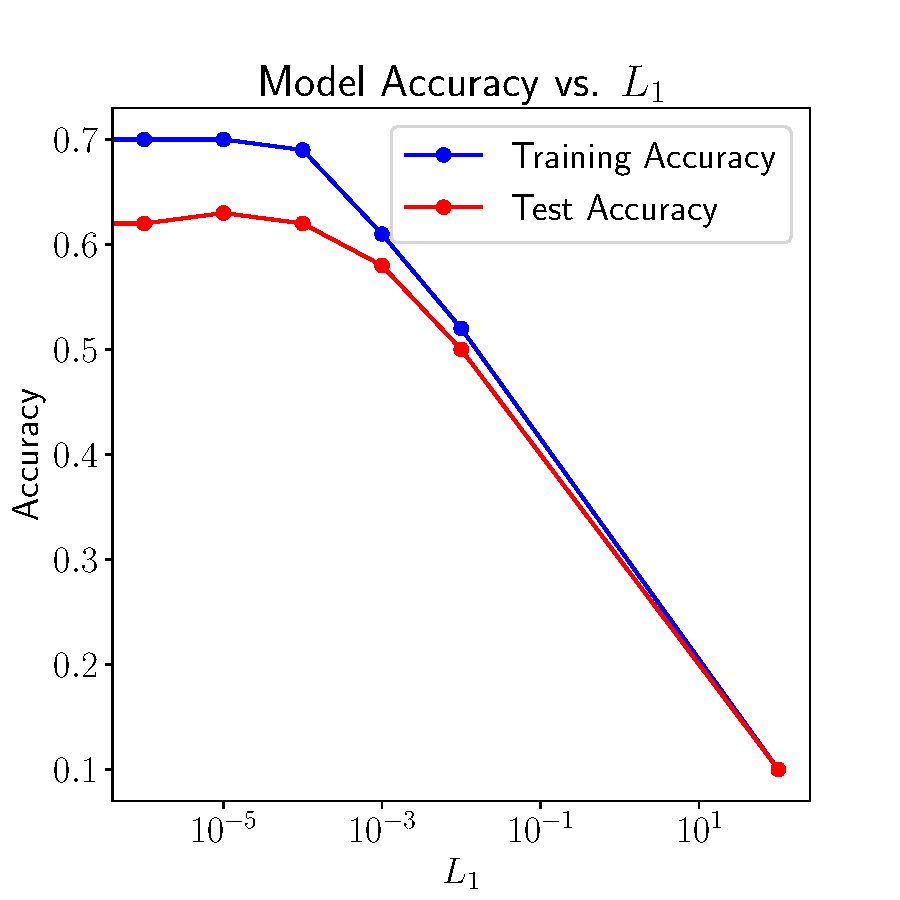
\includegraphics[width=0.49\textwidth]{fig/l1-v-accuracy.pdf}
    \par\end{centering}
    \caption{\label{fig:l1-v-acc}
    A comparison of accuracy on the train and test sets for different $L_1$ regularization weights. The model is trained on 20K samples.}
\end{figure}

Figure \ref{fig:iibiv-acc-loss} presents plots of the `histories' of the training losses and accuracies on training/validation data
for a sequence of models with $L_1\in \{ 0.0,0.00001,0.01,100 \}$.

After 20 epochs the model with $L_1=0.00001$ had a train loss below val loss,
and train accuracy above val accuracy,
which indicates over-fitting,
but the model trained with $L_1=0.01$ exhibits an opposite pattern,
where val score is better than the train score.
However, while the model with $L_1=0.00001$ shows more signs of being fitted too closely to the training data,
the accuracy of the model on validation set is better than the accuracy of the more regularized model, $L_1=0.01$.

While the $L_1$ regularization gives a tool to tweak our preference, i.e. whether
higher accuracy or better generalization is more important to us, it is limited in
that accuracy and generalization might have to be traded off against each other.
We can't get both through tuning $L_1$ alone.
Increasing the amount of training data, on the other hand, helps mitigate overfitting
and gives better performance.


\begin{figure}
    \begin{centering}
        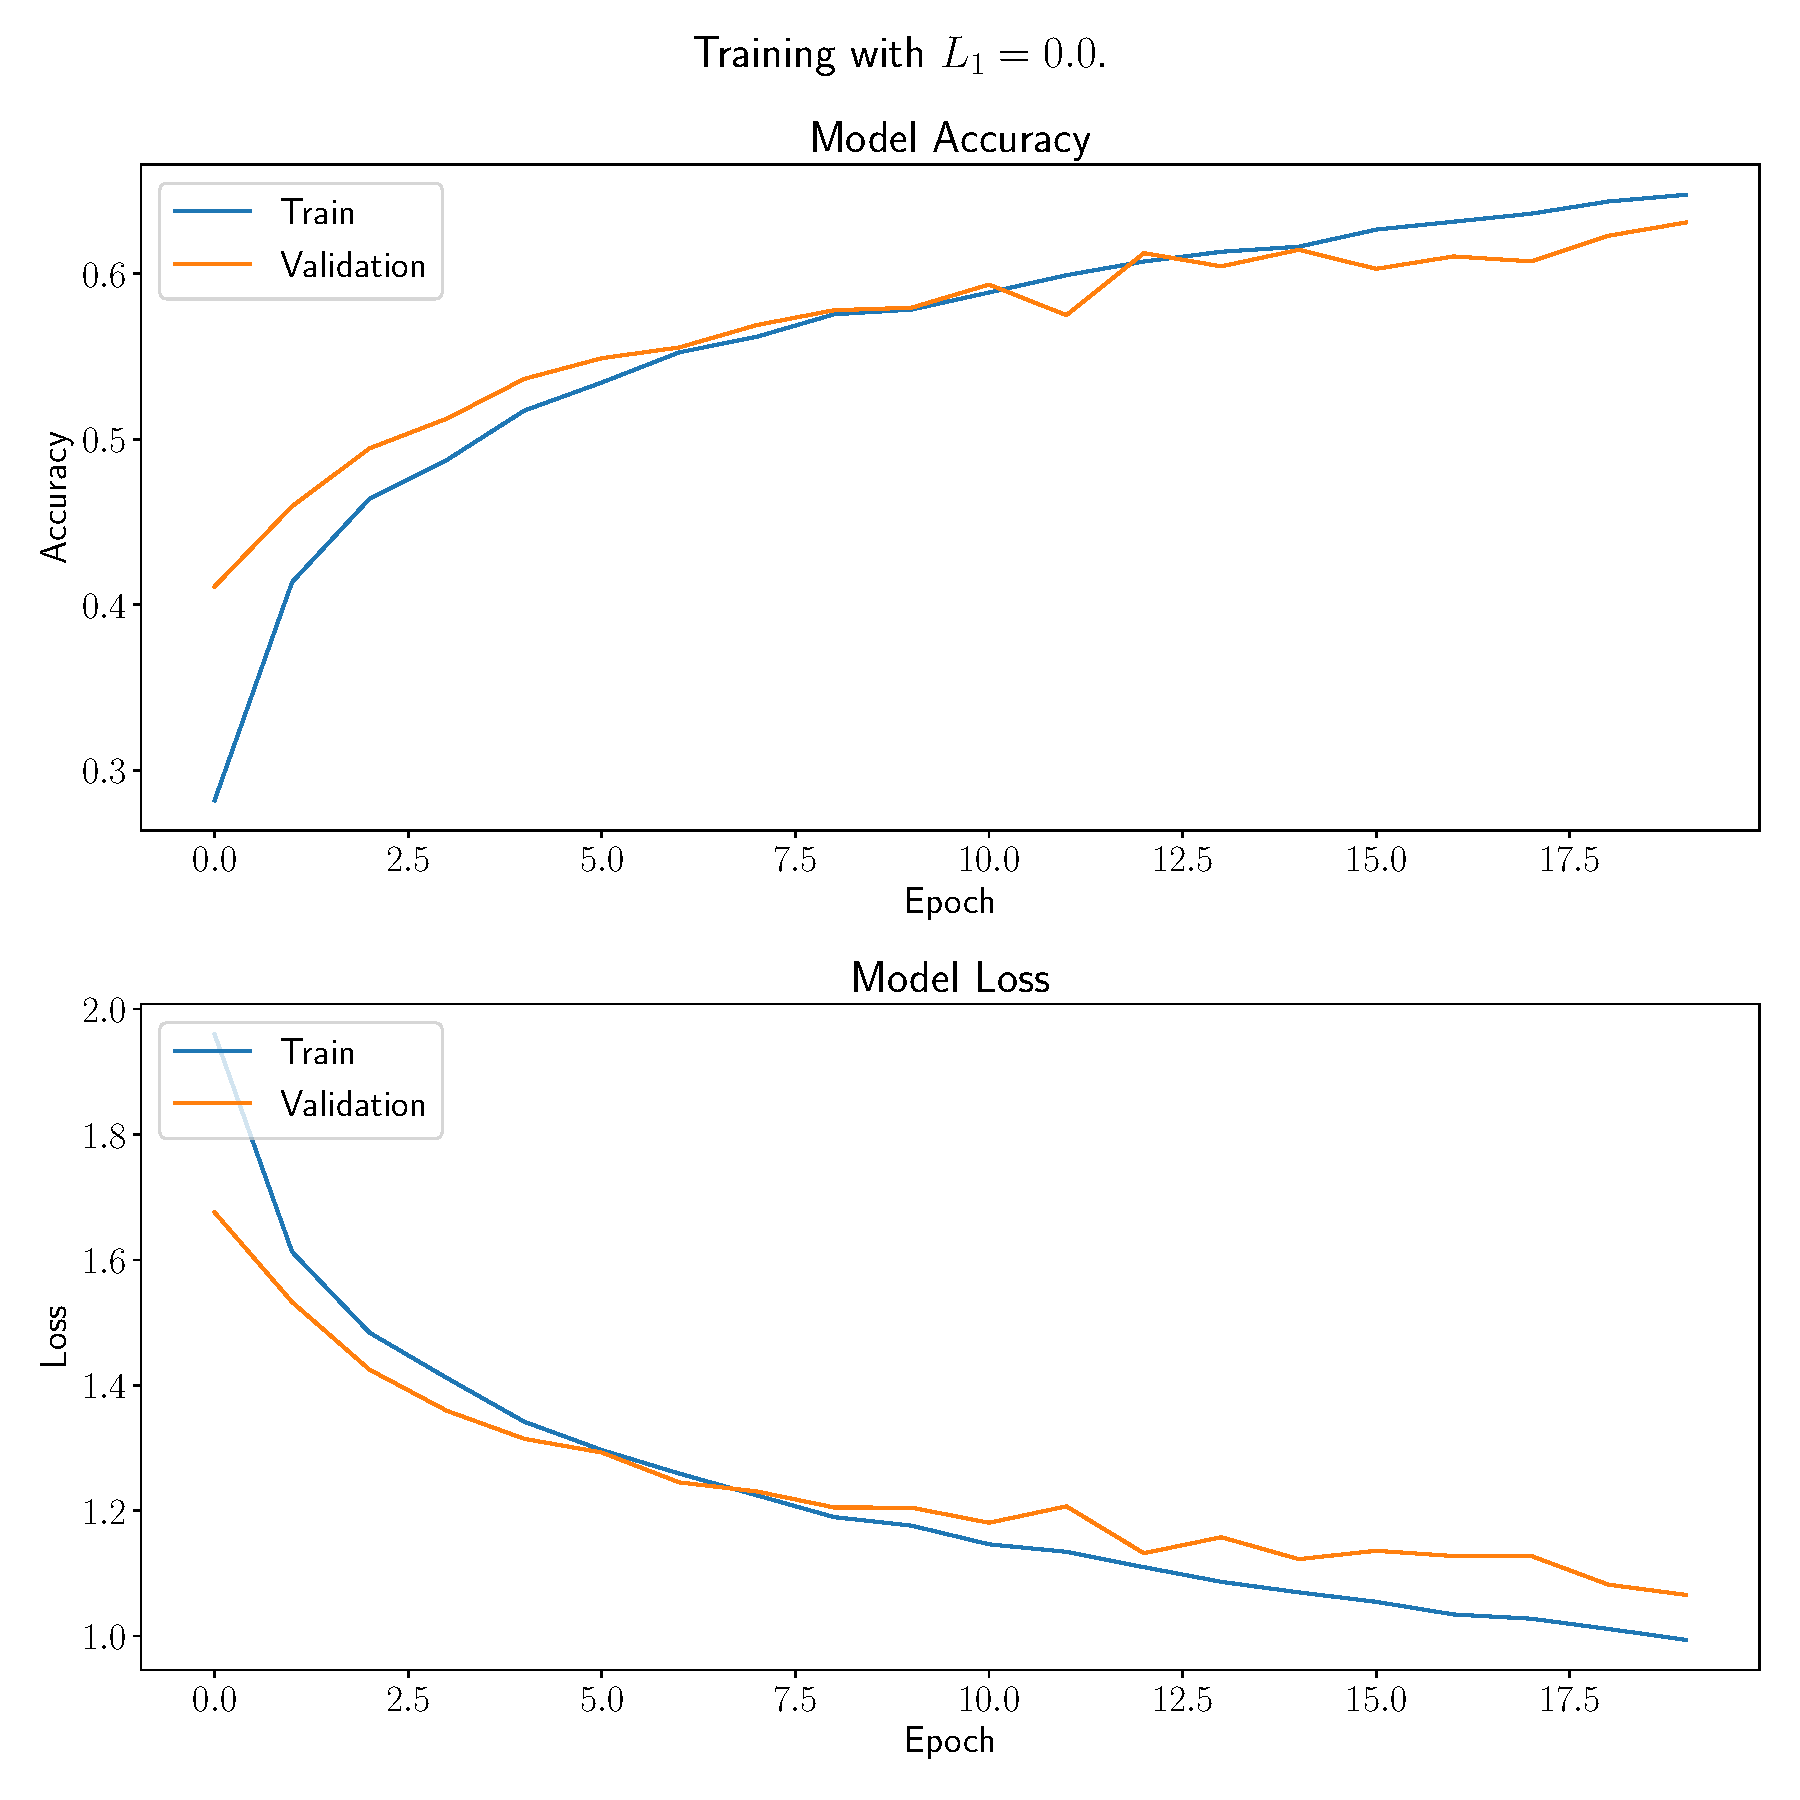
\includegraphics[width=0.49\textwidth]{exp/iibiv/0.0.acc-loss.pdf}
        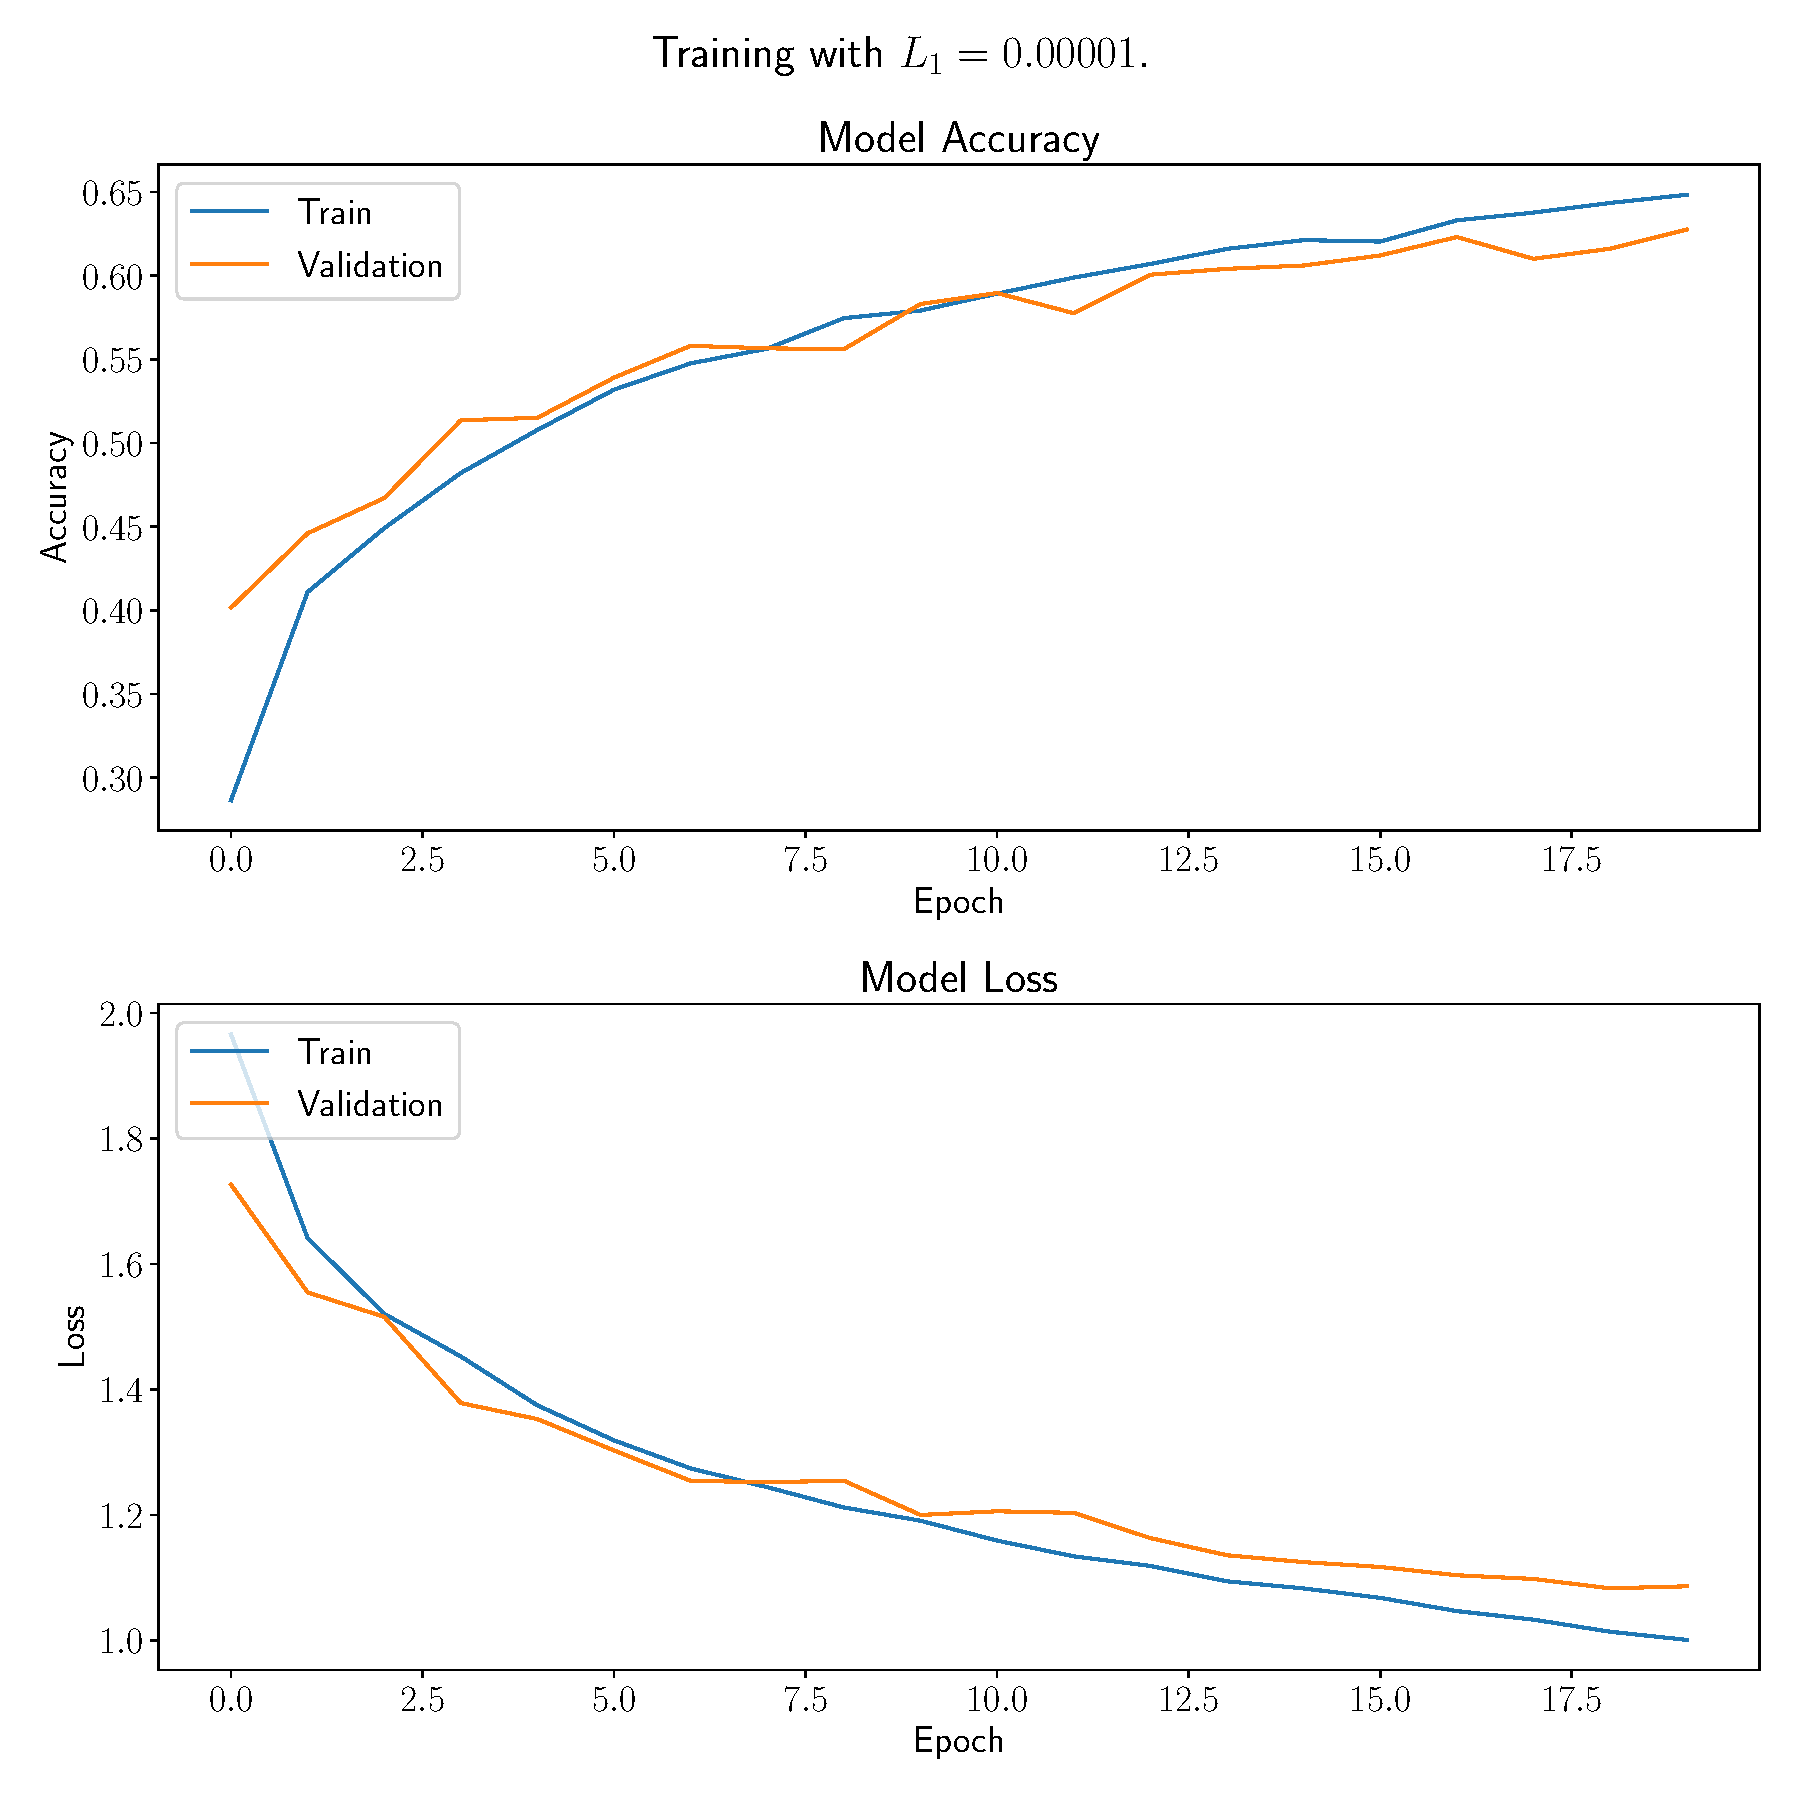
\includegraphics[width=0.49\textwidth]{exp/iibiv/0.00001.acc-loss.pdf}
    \par\end{centering}
    \begin{centering}
        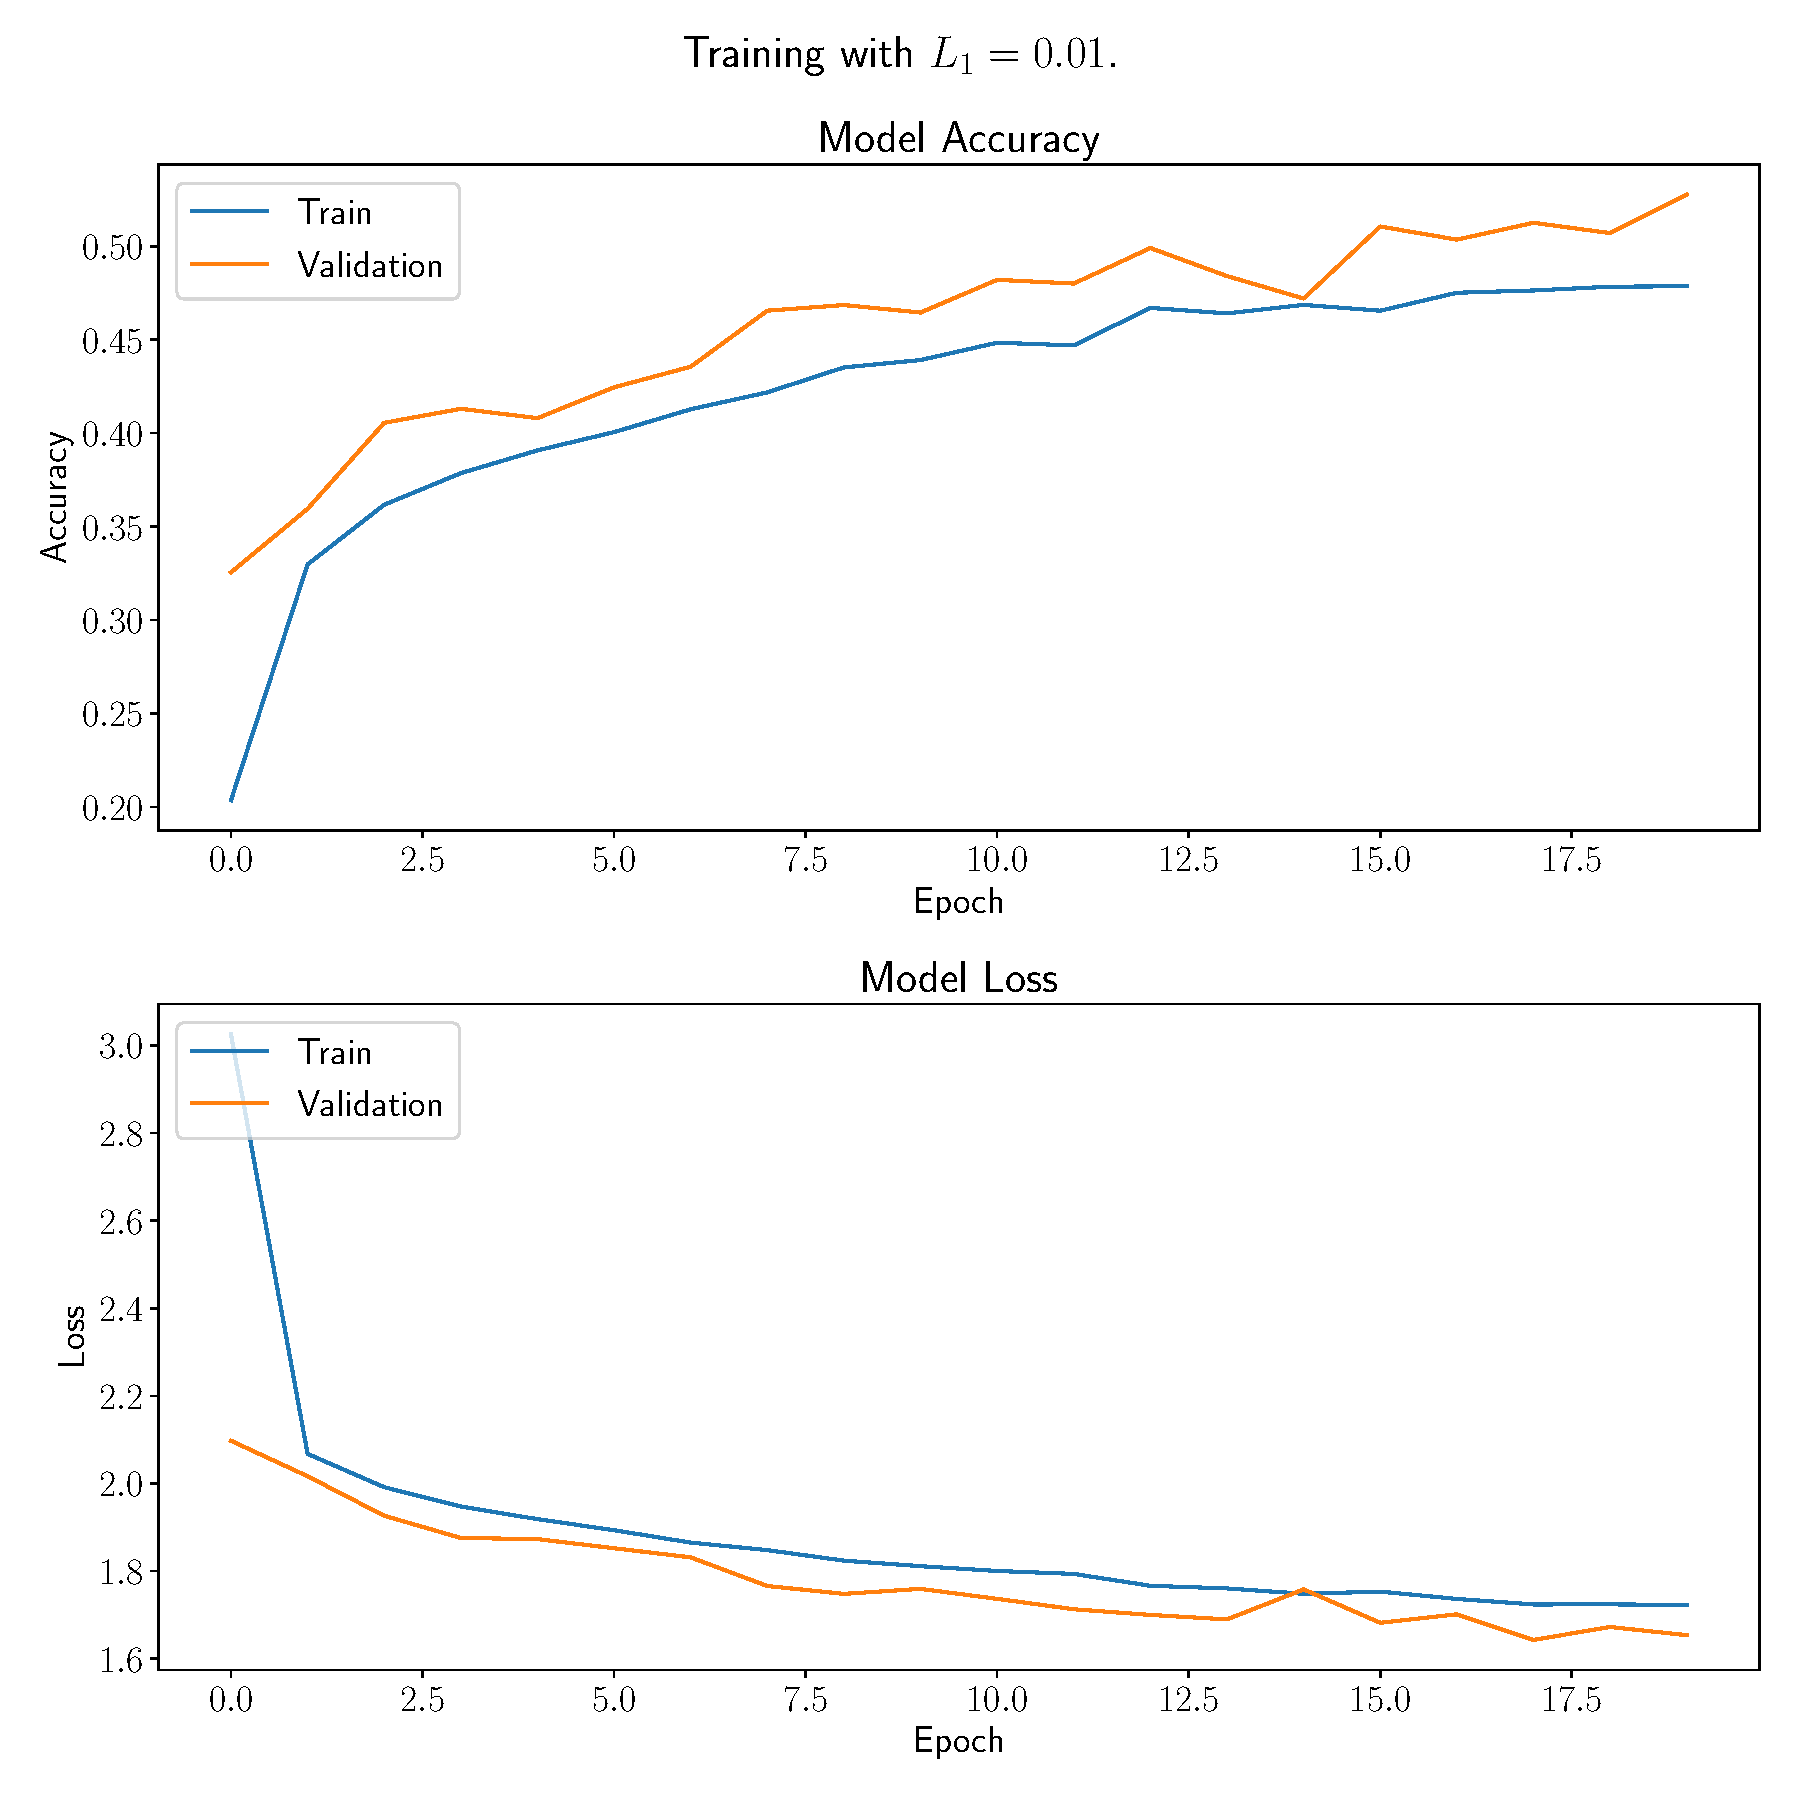
\includegraphics[width=0.49\textwidth]{exp/iibiv/0.01.acc-loss.pdf}
        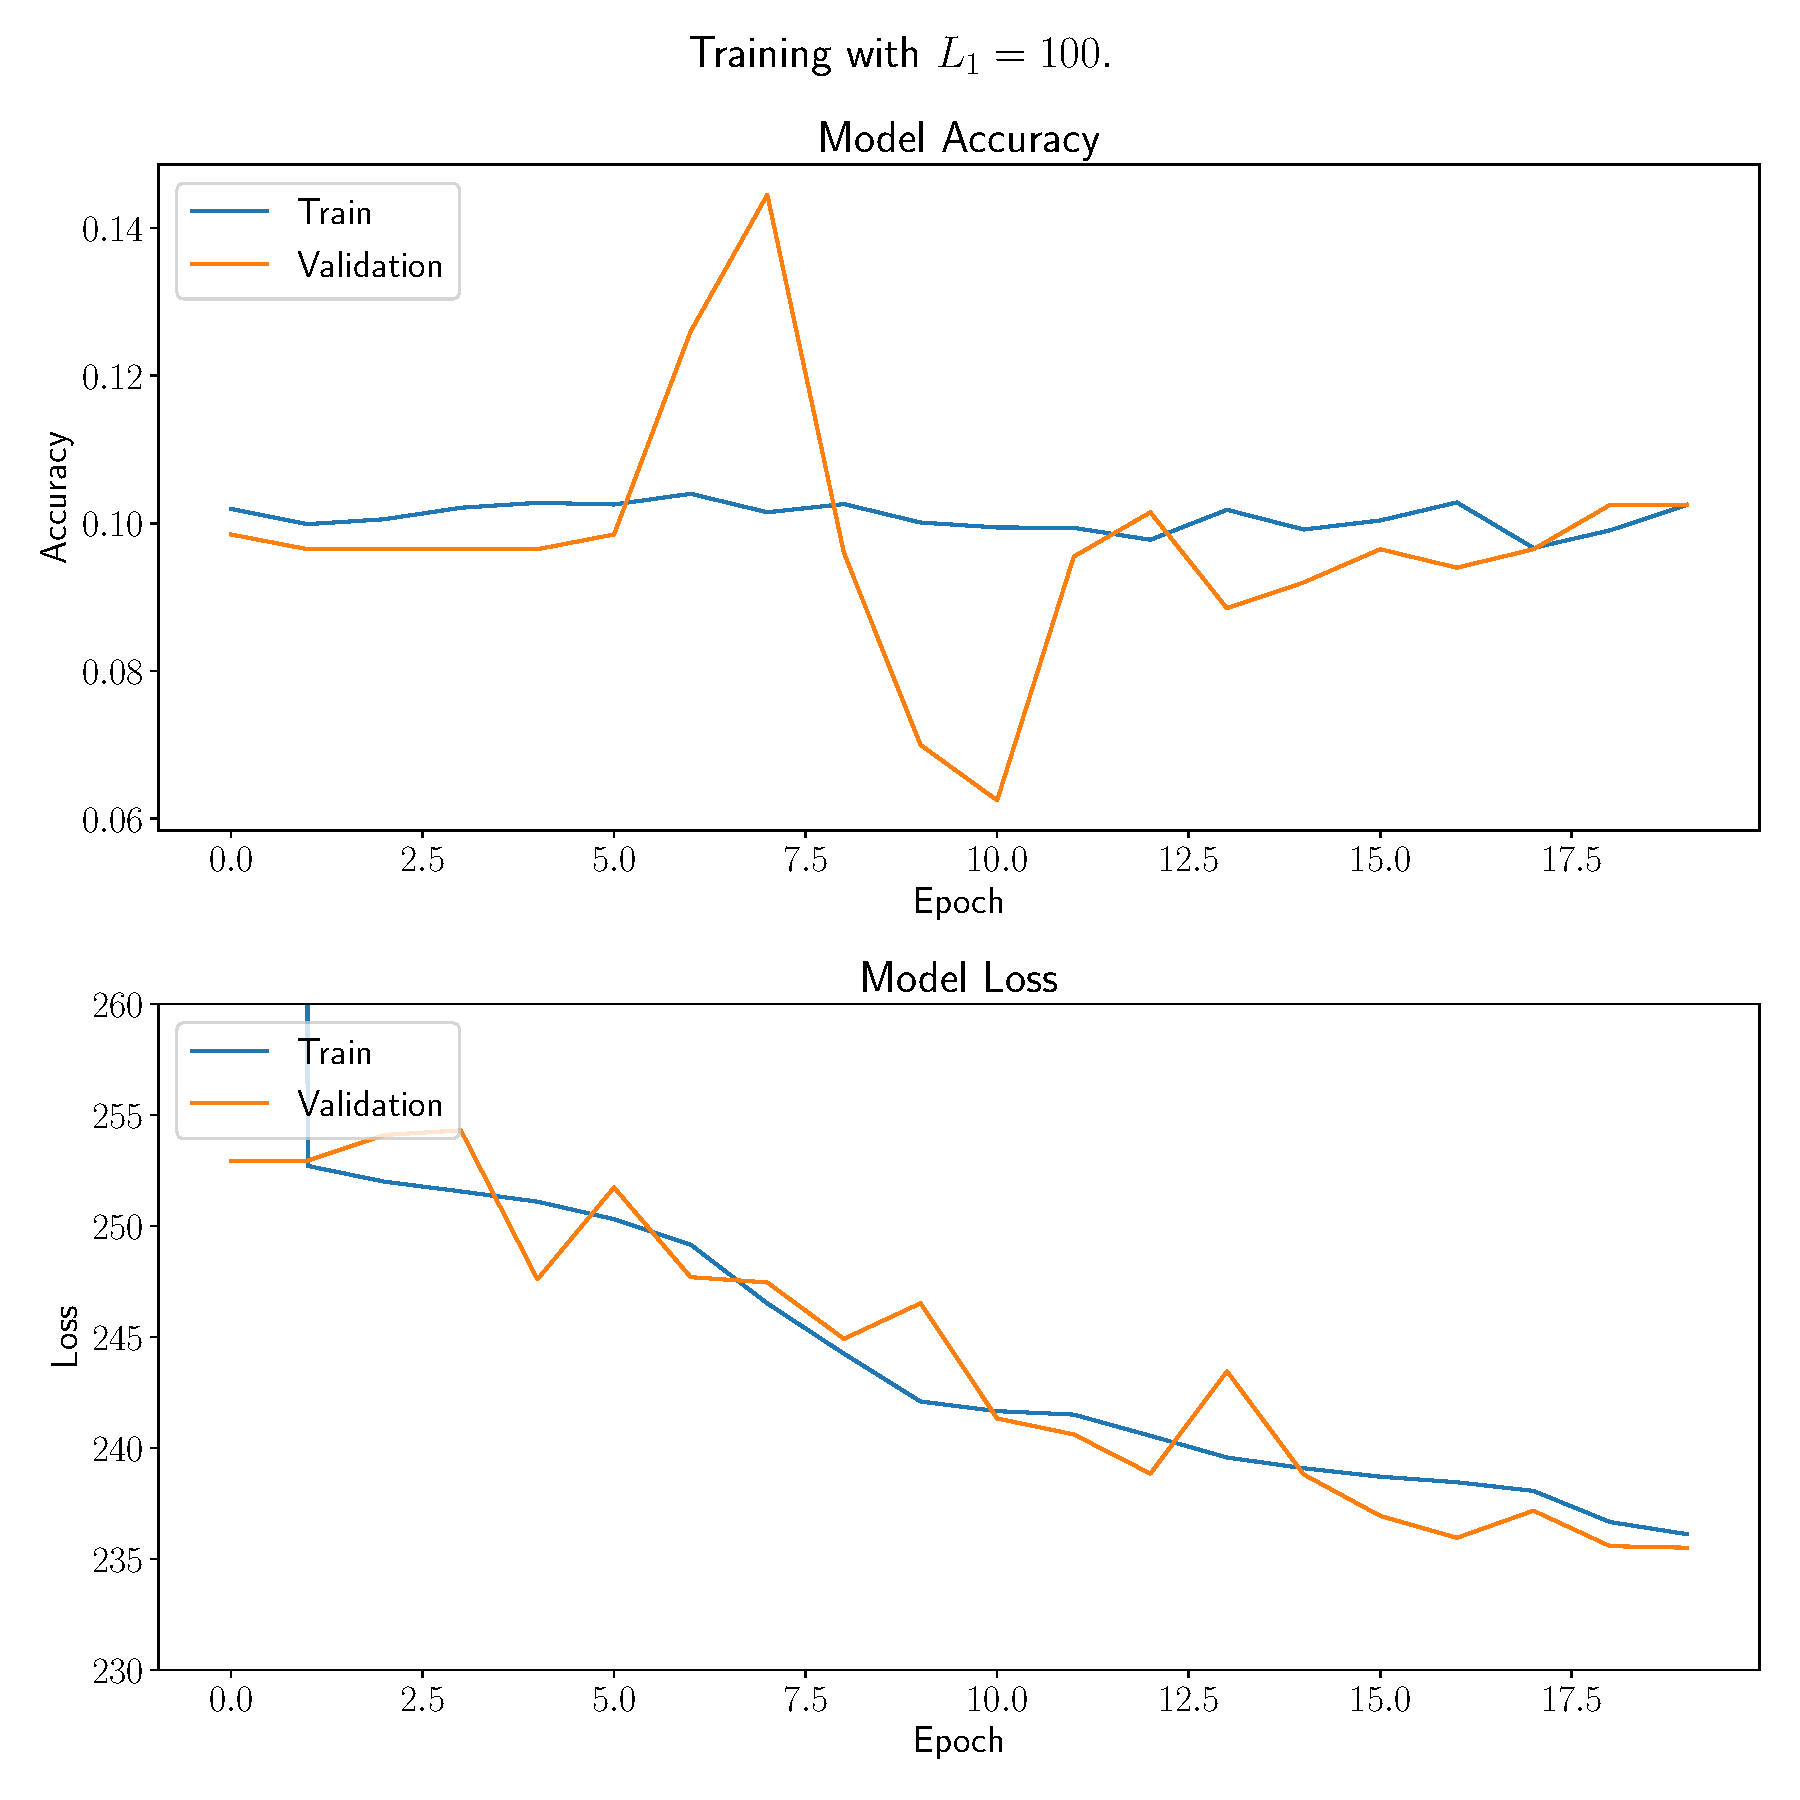
\includegraphics[width=0.49\textwidth]{exp/iibiv/100.acc-loss-lim.pdf}
    \par\end{centering}
    \caption{\label{fig:iibiv-acc-loss}A comparison of accuracy/loss on 
    training/test data from epochs 1 to 20 for different
    $L_1$ regularization terms, $0.0,0.00001,0.01,1000$.
    Each model is trained on 20K training samples.}
\end{figure}

\subsection{(ii) (c)}
The model described for parts (ii) (b) (i)-(iv) above
used 4 layers alternating between stride of (1,1) and (2,2).
The effect of the (2,2) stride layers is that the output tensor's width and height are halved 
(while the `depth' of the tensor is determined by the number of filters).
In this section we compare the stride technique to a model that instead uses max-pooling (2,2)
layers to reduce the dimensionality.
Each layer that had a stride of (2,2) is given a stride of (1,1) and another MaxPooling2D layer
is added to follow that layer.
This MaxPooling2D model has 37146 parameters,
the same number as the model using strided layers.
There is no change to the number of parameters because;
1. the Conv2D layer's number of parameters is independent of the stride
2. the MaxPooling2D layer has no parameters.

% grep -rn timing-50000* -e .
% timing-50000-extra-layers.txt:1:  50000,22.20852756500244
% timing-50000-max-pool.txt:1:      50000,25.55734395980835
% timing-50000.txt:1:               50000,22.167577266693115

The MaxPooling2D version of the model took about
25 seconds to train on 50000 samples (on an A4000 GPU),
whereas the strided version took
about 22 seconds on the same machine (both run at different times of course).
Figure \ref{fig:timing} shows a comparison of training time of the max-pool and strided models.
In general the max-pool approach is slower to train.
The reason the strided version is faster to train is
that the kernel's stride results in skipping a proportion of
the calculations for the forward pass.
With a stride of 2 in both directions the number of times the kernel
is multiplied element-wise by the corresponding slice of the input tensor is
$1/4$ so many as with a stride of 1 in both directions.
The max-pool version also happens to have 2 additional
layers, but this is {\em not} a significant factor in the increased training time.


% strided test 50000 l1=0.0001
% accuracy                           0.70     10000
% macro avg       0.71      0.70      0.70     10000
% weighted avg       0.71      0.70      0.70     10000

% max-pool test 50000 l1=0.0001
% accuracy                           0.74     10000
% macro avg       0.74      0.74      0.74     10000
% weighted avg       0.74      0.74      0.74     10000
The max-pool version achieves the better accuracy of 74\% when trained on 50K samples,
compared to 70\% using the strided architecture.
The aggregated precision, recall, and f1 scores don't
reveal any further differences between the model
architecture's performances and are not reported here for brevity.
Accuracies on 5K samples are compared in Table \ref{tab:max-pool-vs-stride}.

Both models have uneven accuracies on the different classes, i.e. some classes are harder than others, but again not
much interesting is revealed about the differences between the models from the confusion matrices, so they are not reproduced here.

\begin{table}[h]
    \centering
    \begin{tabular}{|l|c|c|}
    \hline
    \textbf{Metric}       & \textbf{MaxPooling2D} & \textbf{stride=(2,2)} \\ \hline
    train accuracy &           66\%            &           62\%          \\ \hline
    test accuracy  &           54\%            &           50\%          \\ \hline
    \end{tabular}
    \caption{Comparison of model performance with MaxPooling2D and stride=(2,2), both using $L_1=0.0001$ and 5K training samples.}
    \label{tab:max-pool-vs-stride}
\end{table}

\subsection{(ii) (d)}
In this section, we make the model deeper and explore the impact on performance, training time, and overfitting.
The model architecture from part (b) (iii) is adjusted by adding two Conv2D layers to the start of
the pipeline, the first with stride=(1,1) and 8 filters, the second with stride=(2,2) and 8 filters,
 both with padding=`same'.
This model has a smaller number of parameters than the model from (b) (iii) because the first two layers reduce the dimensionality while using fewer filters.
With the two extra ConvNet layers the model now has a total of 23314 trainable parameters.
The training time is pretty much the same, as seen in Figure \ref{fig:timing}.

The performance of three model architectures are compared in Table \ref{tab:d-acc}.
It's found that the two extra-layers at the start make the accuracy worse, while the max-pooling architecture gives the best accuracy of 74\%.

The extra layers seem to be causing the model to overfit to the data because the accuracy on the training data is about the same for the strided version and the version with extra layers,
but the accuracy on the test data drops to 65\% when the extra layers are added.

By increasing the depth of the max-pooling variant, adding an extra module (2 Conv2D and  1 MaxPooling2D), we can achieve a better overall accuracy of 77\%,
as seen in Table \ref{tab:d-acc}, but going to 4 total modules leads to significant overfitting. Already with just 3 max-pooling modules we see a greater amount of overfitting,
with 85\% accuracy on train and 77\% accuracy on test.

The impact of increasing the depth in this way on the time taken to train is not clear, as seen in Table \ref{tab:d-time}.

\begin{table}[h]
    \centering
    \caption{\label{tab:d-acc}Accuracies for different neural network configurations over a dataset of 50,000 samples with $L_1$ regularization of 0.0001 and 20 epochs.
    MP means max-pooling, and the number of modules are shown. The third max pooling module has 64 filters, the fourth has 128 filters.
    }
    \begin{tabular}{|l|c|c|c|c|c|}
    \hline
     & Strided & Extra-Layers & MP 2 Modules & MP 3 Modules & MP 4 Modules \\ \hline
    Train Accuracy & 0.75 & 0.74 & 0.78 & 0.85 & 0.91 \\ \hline
    Test Accuracy & 0.70 & 0.65 & 0.74 & 0.77 & 0.76 \\ \hline
    \end{tabular}
\end{table}

\begin{table}[h]
    \centering
    \caption{\label{tab:d-time}Time to train 20 epochs on 50000 samples with deeper and deeper max-pool architectures.}
    \begin{tabular}{|l|c|c|c|}
    \hline
    & Max-Pooling 2 Modules & Max-Pooling 3 Modules & Max-Pooling 4 Modules \\ \hline
    training time (seconds) & 33.46 & 30.09 & 34.14  \\ \hline
    \end{tabular}
\end{table}
    

While additional layers can improve model performance to a point,
they also bring a higher risk of overfitting.
We saw in part (ii) (b) that more data is effective at mitigating overfitting,
but adding more data also increases training time.
It was surprising to see that the increased depth did not increase training time in this case,
but this may have been a fluke or due to an unfair experiment since it was run on a personal desktop.

% train: strided, 50000 samples, l1=0.0001, epochs 20
% accuracy                           0.75     49999
% test: strided, 50000 samples, l1=0.0001, epochs 20
% accuracy                           0.70     10000

% train: max-pooling, 50000 samples, l1=0.0001, epochs 20
% accuracy                           0.78     49999
% test: max-pooling, 50000 samples, l1=0.0001, epochs 20
% accuracy                           0.74     10000

% train: extra-layers, 50000 samples, l1=0.0001, epochs 20
% accuracy                           0.74     49999
% test: extra-layers, 50000 samples, l1=0.0001, epochs 20
% accuracy                           0.65     10000

% train: max-pool-extra, 50000 samples, l1=0.0001, epochs 20
% accuracy                           0.85     49999
% test: max-pool-extra, 50000 samples, l1=0.0001, epochs 20
% accuracy                           0.77     10000

% train: max-pool-extra-2, 50000 samples, l1=0.0001, epochs 20
% accuracy                           0.91     49999
% test: max-pool-extra-2, 50000 samples, l1=0.0001, epochs 20
% accuracy                           0.76     10000


\end{document}
